\documentclass[11pt]{article}

% ========== Packages ==========
\usepackage[a4paper,margin=1in]{geometry}
\usepackage{amsmath,amssymb,mathtools}
\usepackage{bm}
\usepackage{graphicx}
\usepackage{tikz}
\usepackage{booktabs,tabularx,array}
\newcolumntype{L}[1]{>{\raggedright\arraybackslash}p{#1}}
\usepackage{siunitx}
\usepackage{hyperref}
\usepackage[nameinlink]{cleveref}
\usepackage{xcolor}
\usepackage{microtype}
\usepackage{enumitem}

% ========== Macros (minimal, extend as needed) ==========
\newcommand{\Geff}{g^{\mathrm{eff}}_{\mu\nu}}
\newcommand{\Geffinv}{g_{\mathrm{eff}}^{\mu\nu}}
\newcommand{\geff}{g_{\mathrm{eff}}}
\newcommand{\Mpl}{M_{\mathrm{Pl}}}
\newcommand{\Boxg}{\Box_{g_{\mathrm{eff}}}}
\newcommand{\PofX}{P(X)}
\newcommand{\dd}{\mathrm{d}}
\newcommand{\mpl}{M_{\mathrm{Pl}}}
\newcommand{\calO}{\mathcal{O}}

\crefname{section}{Sec.}{Secs.}
\crefname{appendix}{App.}{Apps.}
\crefname{figure}{Fig.}{Figs.}
\crefname{table}{Table}{Tables}

% ========== Title ==========
\title{Proto--Field Gravity V:\\
Emergent Spin--2 Sector and Composite Graviton}
\author{Moeidh M.~Hanash}
\date{\today}

\begin{document}
\maketitle

\begin{abstract}
We investigate the microscopic origin of the tensor sector in the proto--field
gravity model (PFGM), where spacetime geometry and its kinetic term emerge from
a single real scalar field with a rank--one disformal composite metric
\( g^{\rm eff}_{\mu\nu}[\Phi] = \eta_{\mu\nu} + \alpha\,\partial_\mu\Phi\,\partial_\nu\Phi \).
Building on previous work where an Einstein--Hilbert term and higher--curvature
corrections are induced by integrating out proto--field fluctuations, we ask
whether the microscopic Hilbert space actually contains a genuine spin--2
excitation that can be identified as a composite graviton.

On simple but nontrivial backgrounds with a constant proto--field gradient we
construct a composite metric fluctuation operator
\( h_{\mu\nu}[\Phi] \equiv \delta g^{\rm eff}_{\mu\nu}[\Phi] \) and derive
its two--point function from the quadratic proto--field action.  We show that
the corresponding momentum--space correlator admits a spin decomposition with a
massless spin--2 pole of positive residue in the transverse--traceless sector,
while scalar admixtures are either massive or parametrically suppressed in the
infrared.  In the induced--gravity window where the Einstein--Hilbert term
dominates over \(R^2\) and \(C^2\) operators, the linearised equations of motion
for this TT sector reduce to an Einstein--like wave equation sourced by the
standard stress--energy tensor, up to controlled higher--derivative corrections.

These results demonstrate that PFGM supports an emergent composite graviton
with effective dynamics indistinguishable from general relativity at long
wavelengths, providing a concrete microscopic realisation of a massless
spin--2 mode built from a single scalar proto--field.
\end{abstract}


\tableofcontents

% =========================================================
\section{Introduction}
\label{sec:intro}

The proto--field gravity model (PFGM) proposes that both spacetime geometry and
its dynamical kinetic term emerge from a single real scalar ``proto--field''
propagating on a fixed Minkowski background.  The effective geometry is
encoded in a rank--one disformal composite metric
\begin{equation}
  g^{\rm eff}_{\mu\nu}[\Phi] = \eta_{\mu\nu}
  + \alpha\,\partial_\mu\Phi\,\partial_\nu\Phi,
\end{equation}
and matter is minimally coupled to \(g^{\rm eff}_{\mu\nu}\).  Previous work has
shown that fluctuations of the proto--field can induce an Einstein--Hilbert
term and higher--curvature corrections for \(g^{\rm eff}_{\mu\nu}\), with
phenomenologically acceptable parameters and a viable weak--field limit.  In
particular, the PFGM framework has been tested against post--Newtonian
constraints, binary dynamics, and mesoscopic dark--matter phenomenology in a
series of companion papers.

A key conceptual question, however, remains open: what is the microscopic
origin of the tensor sector?  At the level of the induced gravitational
effective action, the theory contains an Einstein--Hilbert term and behaves
like general relativity in the infrared, but this does not by itself guarantee
that the underlying Hilbert space of the proto--field theory contains a
genuine massless spin--2 excitation.  In other words, we would like to know
whether there exists a composite operator built from \(\Phi\) whose
two--point function exhibits the characteristic tensor projector structure and
massless pole of a graviton, and whether this emergent spin--2 mode obeys
Einstein--like dynamics in the regime where the induced Einstein--Hilbert term
dominates.

The purpose of this paper is to address this microscopic question within the
PFGM setup.  Working on simple but nontrivial backgrounds with a constant
proto--field gradient, we construct a composite metric fluctuation operator
\(h_{\mu\nu}[\Phi]\equiv \delta g^{\rm eff}_{\mu\nu}[\Phi]\), derive its
two--point function from the quadratic proto--field action, and analyse its
spin content.  We show that the transverse--traceless sector of the
\(\langle h h\rangle\) correlator contains a massless spin--2 pole with
positive residue, while scalar admixtures are either massive or suppressed in
the infrared.  We then connect this composite operator to the induced
Einstein--Hilbert action and demonstrate that, in the appropriate low--energy
window, the linearised equations of motion for the transverse--traceless
sector reduce to an Einstein--like wave equation sourced by the standard
stress--energy tensor.

\subsection{Motivation and context}
\label{subsec:intro_motivation}

Emergent and induced gravity scenarios have long sought to explain the
Einstein--Hilbert action and its massless spin--2 excitations as effective
phenomena arising from more fundamental microscopic degrees of freedom.
Examples range from Sakharov--type induced gravity to analogue gravity systems
and various compositeness proposals for the graviton.  The PFGM framework adds
a particularly economical realisation: a single scalar field with a disformal
composite metric and a healthy higher--derivative microscopic action.  In
earlier work, the focus was on deriving the induced gravitational action,
establishing the existence of a viable Einstein--Hilbert term and constraining
higher--curvature operators using post--Newtonian and strong--field tests.

From this perspective, the present paper fills an important conceptual gap.  It
provides a concrete demonstration that the scalar proto--field can support an
emergent tensor sector whose long--wavelength dynamics are indistinguishable
from those of general relativity, and it clarifies how the effective
diffeomorphism invariance of the induced action is realised in terms of
underlying scalar degrees of freedom.

\subsection{Summary of results}
\label{subsec:intro_summary}

An important theme throughout is that the graviton in PFGM appears as a massless spin--2 composite bound state of the scalar proto--field, rather than as a fundamental tensor field.
The main results of this paper can be summarised as follows:
\begin{itemize}[leftmargin=*]
  \item We construct a composite metric fluctuation operator
  \(h_{\mu\nu}[\Phi]\equiv \delta g^{\rm eff}_{\mu\nu}[\Phi]\) on backgrounds
  with a constant proto--field gradient and derive the quadratic action for
  proto--field fluctuations propagating on the corresponding effective metric.
  \item Using the resulting propagator, we compute the momentum--space
  two--point function \(\langle h_{\mu\nu}(k)\,h_{\rho\sigma}(-k)\rangle\) and
  decompose it into standard spin projectors.  We show that the
  transverse--traceless sector exhibits a massless spin--2 pole with positive
  residue, while scalar components are either massive or parametrically
  suppressed in the infrared.
  \item We relate the normalisation of the massless spin--2 pole to the
  effective Planck scale appearing in the induced Einstein--Hilbert term,
  thereby identifying the composite graviton of PFGM with the tensor mode of
  the induced gravitational effective action.
  \item In the window where the induced Einstein--Hilbert term dominates over
  higher--curvature corrections, we derive the linearised equations of motion
  for the transverse--traceless sector and show that they reduce to an
  Einstein--like wave equation sourced by the standard stress--energy tensor,
  with controlled higher--derivative corrections.
  \item We discuss degrees of freedom and emergent gauge structure, clarifying
  how the two physical tensor polarisations arise from the underlying scalar
  dynamics and under which conditions the effective diffeomorphism invariance
  is a good symmetry.
\end{itemize}

\subsection{Organisation of the paper}
\label{subsec:intro_organisation}

The remainder of the paper is organised as follows.
In \cref{sec:setup} we briefly review the microscopic proto--field action and
the disformal composite metric, and summarise the induced Einstein--Hilbert
term and its regime of validity.  In \cref{sec:backgrounds} we introduce the
backgrounds of interest and the fluctuation decomposition of the proto--field.
In \cref{sec:composite_fluctuations} we construct the composite metric
fluctuation operator and derive the quadratic action and propagator for the
proto--field.  In \cref{sec:spin2_propagator} we compute the composite
\(\langle h h\rangle\) correlator, perform the spin decomposition, and isolate
the massless spin--2 pole.  In \cref{sec:linearised_dynamics} we connect this
composite graviton to the induced Einstein--Hilbert action and derive the
linearised equations of motion and coupling to matter in the infrared.  In
\cref{sec:DOF_gauge} we discuss degrees of freedom and emergent gauge
structure.  Finally, in \cref{sec:discussion,sec:outlook} we place our results
in the broader context of emergent gravity scenarios and outline directions
for future work.

\begin{figure}[t]
  \centering
  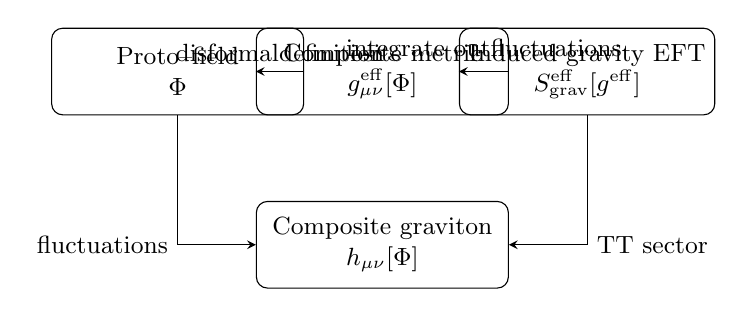
\begin{tikzpicture}[node distance=2.6cm, >=stealth, font=\small]
    \tikzstyle{box}=[draw, rounded corners, align=center,
      minimum width=3.2cm, minimum height=1.1cm]
    \node[box] (phi) {Proto--field\\$\Phi$};
    \node[box, right of=phi] (metric) {Composite metric\\$g^{\rm eff}_{\mu\nu}[\Phi]$};
    \node[box, right of=metric] (EH) {Induced gravity EFT\\$S_{\rm grav}^{\rm eff}[g^{\rm eff}]$};
    \node[box, below of=metric, node distance=2.2cm] (grav) {Composite graviton\\$h_{\mu\nu}[\Phi]$};

    \draw[->] (phi) -- node[above]{disformal\\definition} (metric);
    \draw[->] (metric) -- node[above]{integrate out\\fluctuations} (EH);
    \draw[->] (phi) |- node[left]{fluctuations} (grav);
    \draw[->] (EH) |- node[right]{TT sector} (grav);
  \end{tikzpicture}
  \caption{Schematic structure of the proto--field gravity model. A single scalar
  proto--field $\Phi$ defines a composite metric $g^{\rm eff}_{\mu\nu}[\Phi]$
  and, upon integrating out fluctuations, induces an Einstein--Hilbert--dominated
  effective action. The composite graviton $h_{\mu\nu}[\Phi]$ appears as a bound
  state in the transverse--traceless sector of the composite metric fluctuations.}
  \label{fig:schematic_PFGM}
\end{figure}

\section{Proto--field setup and composite metric}
\label{sec:setup}

In this section we briefly review the microscopic proto--field action, the
disformal composite metric to which matter is coupled, and the structure of the
induced gravitational effective action.  The emphasis is on fixing notation and
summarising those aspects of the setup that are directly relevant for the
emergent spin--2 sector studied in later sections.

\subsection{Microscopic proto--field action}
\label{subsec:setup_action}

The fundamental degree of freedom is a single real scalar field \(\Phi\)
propagating on a fixed Minkowski background \(\eta_{\mu\nu}\).  Its microscopic
action is of \(P(X)\) type, augmented by a stabilising quartic derivative term
that ensures the existence of a healthy band of backgrounds,
\begin{equation}
  S_\Phi = \int \mathrm{d}^4x\,
  \bigg[ P(X) + \frac{\beta_2}{\Lambda^4}
   (\partial_\mu\partial_\nu\Phi\,\partial^\mu\partial^\nu\Phi) \bigg],
  \qquad
  X \equiv -\frac12\,\eta^{\mu\nu}\partial_\mu\Phi\,\partial_\nu\Phi,
\end{equation}
where \(P(X)\) is a smooth function with suitable derivatives in the regime of
interest, \(\beta_2\) is a dimensionless coefficient, and \(\Lambda\) denotes a
microscopic scale controlling the onset of higher--derivative corrections.
The second term is written schematically; in practice only a particular
combination of quartic structures is needed to achieve stability, but its
detailed form will not be important in what follows.

As shown in Refs.~\cite{Hanash:PFGM-I,Hanash:Induced-EH}, the microscopic
parameters of the proto--field theory admit a nonempty region in which small
fluctuations around constant--gradient backgrounds are free of ghosts and
gradient instabilities.  In terms of the \(P(X)\) sector alone this typically requires
\begin{equation}
  P'(X_0) > 0,
  \qquad
  P'(X_0) + 2X_0 P''(X_0) > 0,
\end{equation}
where \(X_0\) is the value of \(X\) evaluated on the background solution
\(\Phi_0\).  The quartic term controlled by \(\beta_2\) can then be tuned to
ensure hyperbolicity and to avoid strong coupling in the fluctuation sector,
as discussed in more detail in the induced--gravity analysis.

\subsection{Disformal composite metric and effective geometry}
\label{subsec:setup_metric}

The effective geometry seen by matter is encoded in a rank--one disformal
composite metric built from the proto--field gradient,
\begin{equation}
  g^{\rm eff}_{\mu\nu}[\Phi]
  = \eta_{\mu\nu} + \alpha\,\partial_\mu\Phi\,\partial_\nu\Phi,
\end{equation}
with \(\alpha\) a constant parameter of mass dimension \(-4\).  This metric is
invertible as long as \(1 + \alpha\,\partial_\lambda\Phi\,\partial^\lambda\Phi
\neq 0\).  For later use it is convenient to write the inverse metric as
\begin{equation}
  g_{\rm eff}^{\mu\nu}
  = \eta^{\mu\nu}
  - \frac{\alpha}{1+\alpha\,(\partial\Phi)^2}
    \,\partial^\mu\Phi\,\partial^\nu\Phi,
  \qquad
  (\partial\Phi)^2 \equiv \eta^{\rho\sigma}\partial_\rho\Phi\,\partial_\sigma\Phi,
\end{equation}
and the determinant as
\begin{equation}
  \sqrt{-g_{\rm eff}} = \sqrt{-\eta}\,
  \big[1 + \alpha\,(\partial\Phi)^2\big]^{1/2},
\end{equation}
where \(\sqrt{-\eta}=1\) in Cartesian coordinates on Minkowski space.

Matter fields \(\Psi_{\rm m}\) are assumed to be minimally coupled to the
composite metric \(g^{\rm eff}_{\mu\nu}\),
\begin{equation}
  S_{\rm m}[g^{\rm eff},\Psi_{\rm m}]
  = \int \mathrm{d}^4x\,\sqrt{-g_{\rm eff}}\,
    \mathcal{L}_{\rm m}\big(g^{\rm eff}_{\mu\nu},\Psi_{\rm m}\big),
\end{equation}
so that their stress--energy tensor is defined in the usual way with respect to
\(g^{\rm eff}_{\mu\nu}\).  This choice ensures that any emergent tensor mode
constructed from \(g^{\rm eff}_{\mu\nu}\) will couple universally to matter in
the low--energy regime, provided the induced gravitational action for
\(g^{\rm eff}_{\mu\nu}\) takes the Einstein--Hilbert form.

\subsection{Induced Einstein--Hilbert term and IR effective theory}
\label{subsec:setup_induced_EH}

Integrating out proto--field fluctuations around a given background generates
an effective action for the composite metric \(g^{\rm eff}_{\mu\nu}\).  At
one--loop order, and within the healthy band described above, the leading
geometric terms take the schematic form
\begin{equation}
  S_{\rm grav}^{\rm eff}[g^{\rm eff}]
  = \int \mathrm{d}^4x\,\sqrt{-g_{\rm eff}}\,
    \bigg[ \frac{\Mpl^2}{2}\,R[g^{\rm eff}]
           + c_1 R^2[g^{\rm eff}] + c_2 C^2[g^{\rm eff}]
           + \cdots \bigg],
\end{equation}
where \(R\) is the Ricci scalar, \(C^2\) denotes the square of the Weyl tensor,
\(\Mpl\) is an induced Planck mass, and the ellipsis stands for higher--order
curvature invariants and nonlocal contributions suppressed at low energies.
The coefficients \(\Mpl^2,c_1,c_2,\ldots\) are calculable functions of the
microscopic parameters of the proto--field theory and of the background value
of \(X\).

In the regime where curvatures and momenta are small compared to the scale set
by \(|c_{1,2}|/\Mpl^2\), the Einstein--Hilbert term dominates and the
gravitational dynamics are well approximated by general relativity with
effective Planck mass \(\Mpl\).  Previous work has shown that, for suitable
choices of microscopic parameters, this induced--gravity effective theory
passes standard weak--field and post--Newtonian tests, and admits nontrivial
mesoscopic behaviour relevant to dark--matter phenomenology.  In the present
paper we focus on the microscopic origin of the tensor sector associated with
the induced Einstein--Hilbert term, and in particular on the identification of
a composite graviton operator built from the proto--field.

\section{Backgrounds and fluctuation decomposition}
\label{sec:backgrounds}

To analyse the emergent spin--2 sector it is convenient to work on simple
backgrounds for which the disformal structure of the composite metric is
nontrivial but still amenable to explicit calculation.  In this section we
introduce such backgrounds and set up the background--field split of the
proto--field, preparing the ground for the construction of composite metric
fluctuations in \cref{sec:composite_fluctuations}.

\subsection{Constant-gradient background on Minkowski}
\label{subsec:bg_constant_gradient}

The simplest nontrivial configuration of the proto--field is one with a
constant gradient,
\begin{equation}
  \Phi_0(x) = q_\mu x^\mu,
  \qquad
  q_\mu = \text{const},
\end{equation}
so that \(X\) is constant,
\begin{equation}
  X_0 = -\frac12\,\eta^{\mu\nu}q_\mu q_\nu = \text{const}.
\end{equation}
On such a background the composite metric becomes
\begin{equation}
  \bar g_{\mu\nu}
  \equiv g^{\rm eff}_{\mu\nu}[\Phi_0]
  = \eta_{\mu\nu} + \alpha\,q_\mu q_\nu,
\end{equation}
which is a flat metric related to \(\eta_{\mu\nu}\) by an anisotropic but
spacetime--independent deformation.  Since \(\bar g_{\mu\nu}\) has constant
components, its associated Riemann tensor vanishes and the background is
globally Minkowski in appropriate coordinates, although the light cones of
matter and proto--field fluctuations need not coincide with those of the
original \(\eta_{\mu\nu}\).

Without loss of generality we can work in a frame where the background gradient
is purely timelike,
\begin{equation}
  q_\mu = (q,0,0,0),
\end{equation}
so that
\begin{equation}
  \bar g_{\mu\nu}
  = \mathrm{diag}\big(-(1-\alpha q^2),1,1,1\big),
  \qquad
  q_\mu q^\mu \equiv \eta^{\mu\nu} q_\mu q_\nu = -q^2.
\end{equation}
In this frame the composite metric is manifestly homogeneous and isotropic in
space, and all quantities of interest can be conveniently analysed in Fourier
space with respect to the associated time coordinate and spatial momenta.

\subsection{Cosmological (FRW-like) background}
\label{subsec:bg_FRW}

The constant-gradient background provides a clean playground for the study of
composite spin--2 excitations, but it is also useful to note how the setup
extends to more general, mildly curved backgrounds.  A particularly relevant
case is a homogeneous time--dependent proto--field,
\begin{equation}
  \Phi_0(t), \qquad \partial_i\Phi_0 = 0,
\end{equation}
for which the composite metric takes a spatially homogeneous and isotropic
form,
\begin{equation}
  \mathrm{d}s^2
  = g^{\rm eff}_{\mu\nu}[\Phi_0]\,\mathrm{d}x^\mu\mathrm{d}x^\nu
  = -A(t)\,\mathrm{d}t^2 + B(t)\,\delta_{ij}\,\mathrm{d}x^i\mathrm{d}x^j,
\end{equation}
with lapse and scale--factor functions \(A(t)\) and \(B(t)\) determined by
\(\Phi_0(t)\) and the microscopic parameters.  This defines an effective
Friedmann--Robertson--Walker (FRW)--type geometry for matter and proto--field
fluctuations.

In the present paper we will restrict explicit calculations of the composite
spin--2 propagator to the constant--gradient background, where the effective
metric is flat and momentum--space methods are particularly transparent.
However, the construction of the composite operator and its spin decomposition
can in principle be generalised to slowly varying FRW--like backgrounds, and
we comment on this extension in \cref{app:alt_backgrounds}.

\subsection{Healthy band and stability conditions}
\label{subsec:bg_healthy_band}

As already noted in \cref{subsec:setup_action}, the microscopic parameters of the
proto--field theory can be chosen to lie in the healthy band identified in
Refs.~\cite{Hanash:PFGM-I,Hanash:Induced-EH}, in which small fluctuations are
free of ghosts and gradient instabilities.  On the constant--gradient background
this amounts to requiring that the quadratic action for fluctuations has a
positive--definite kinetic term and a hyperbolic principal symbol with respect
to the composite metric \(\bar g_{\mu\nu}\).

Denoting by \(\chi\) the fluctuation of the proto--field around \(\Phi_0\),
\begin{equation}
  \Phi = \Phi_0 + \chi,
\end{equation}
the quadratic action takes the schematic form
\begin{equation}
  S^{(2)}[\chi;\Phi_0]
  = \frac12\int \mathrm{d}^4x\,\sqrt{-\bar g}\,
     \chi\,\mathcal{D}[\bar g,\Phi_0]\,\chi,
\end{equation}
where \(\mathcal{D}\) is a differential operator whose leading, second--order part has
principal symbol controlled by an effective characteristic metric constructed from
\(\bar g_{\mu\nu}\) and the derivatives of \(P(X)\) evaluated at \(X_0\),
together with contributions from the quartic term.  The healthy--band
conditions translate into positivity constraints on the eigenvalues of this
characteristic metric and on the sign of the kinetic term in the corresponding
Hamiltonian.

In the following sections we will assume that these conditions are satisfied,
so that \(\chi\) admits a well--defined propagator on the constant--gradient
background and can be used to construct a composite metric fluctuation operator
with sensible infrared behaviour.

% =========================================================
\section{Composite metric fluctuations}
\label{sec:composite_fluctuations}

In this section we construct the composite metric fluctuation operator
\(h_{\mu\nu}[\Phi]\) and derive the quadratic action and propagator for the
underlying proto--field fluctuation \(\chi\) on the constant--gradient
background introduced in \cref{subsec:bg_constant_gradient}.  These results
provide the basic input for the analysis of the emergent spin--2 propagator in
\cref{sec:spin2_propagator}.

\subsection{Background-field split and canonical fluctuation}
\label{subsec:fluct_split}

We begin by decomposing the proto--field into a background configuration and a
fluctuation,
\begin{equation}
  \Phi(x) = \Phi_0(x) + \chi(x),
  \qquad
  \Phi_0(x) = q_\mu x^\mu,
\end{equation}
where \(q_\mu\) is a constant timelike vector and \(\chi\) denotes the
fluctuation.  On this background the kinetic invariant
\(X = -\tfrac12 \eta^{\mu\nu}\partial_\mu\Phi\,\partial_\nu\Phi\) takes the
constant value
\begin{equation}
  X_0 = -\frac12\,\eta^{\mu\nu}q_\mu q_\nu,
\end{equation}
and the composite metric reduces to the flat tensor
\(\bar g_{\mu\nu} = g^{\rm eff}_{\mu\nu}[\Phi_0]
 = \eta_{\mu\nu} + \alpha q_\mu q_\nu\) introduced in
\cref{subsec:bg_constant_gradient}.

Expanding the microscopic action \(\int \dd^4x\,\mathcal{L}_\Phi(\Phi)\) to
second order in \(\chi\) and discarding total derivatives yields the quadratic
action
\begin{equation}
  S^{(2)}[\chi;\Phi_0]
  = \frac12\int \mathrm{d}^4x\,\sqrt{-\bar g}\,
     \chi\,\mathcal{D}[\bar g,\Phi_0]\,\chi,
  \label{eq:fluct_quadratic_action}
\end{equation}
where \(\mathcal{D}[\bar g,\Phi_0]\) is a second--order differential operator
whose principal symbol and lower--derivative terms are determined by the
derivatives of \(P(X)\) evaluated at \(X_0\) and by the quartic derivative
coupling \(\beta_2\); explicit expressions are given in
\cref{app:quad_action}.  In the healthy band defined in
\cref{app:quad_dispersion} the eigenvalues of the principal symbol are
positive, so that \(\chi\) defines a single propagating scalar degree of
freedom with a real dispersion relation and no ghosts.

\subsection{Linearised composite metric}
\label{subsec:fluct_linear_metric}

The effective metric depends on \(\Phi\) only through its gradient.  Expanding
\(g^{\rm eff}_{\mu\nu}[\Phi]\) around the constant--gradient background yields
\begin{equation}
  g^{\rm eff}_{\mu\nu}[\Phi]
  = g^{\rm eff}_{\mu\nu}[\Phi_0]
    + \delta g^{\rm eff}_{\mu\nu}[\chi]
    + \delta^2 g^{\rm eff}_{\mu\nu}[\chi]
    + \cdots,
\end{equation}
where the linear term is
\begin{equation}
  \delta g^{\rm eff}_{\mu\nu}[\chi]
  = \alpha\big(
      \partial_\mu\Phi_0\,\partial_\nu\chi
    + \partial_\mu\chi\,\partial_\nu\Phi_0
    \big)
  = \alpha\big(
      q_\mu\,\partial_\nu\chi
    + q_\nu\,\partial_\mu\chi
    \big),
\end{equation}
using \(\partial_\mu\Phi_ = q_\mu\).  We define the linearised composite metric
fluctuation operator
\begin{equation}
  h_{\mu\nu}(x)
  \equiv \delta g^{\rm eff}_{\mu\nu}[\chi](x)
  = \alpha\big(
      q_\mu\,\partial_\nu\chi(x)
    + q_\nu\,\partial_\mu\chi(x)
    \big),
  \label{eq:fluct_h_def}
\end{equation}
which will be the central object in our analysis of the emergent tensor
sector.  Higher--order terms \(\delta^2 g^{\rm eff}_{\mu\nu}[\chi]\) generate
self--interactions among the composite gravitons but do not affect the
tree--level two--point function studied in \cref{sec:spin2_propagator}.

It is convenient to work in momentum space with respect to the background
coordinates associated with \(\bar g_{\mu\nu}\).  Writing
\begin{equation}
  \chi(x) = \int \frac{\mathrm{d}^4k}{(2\pi)^4}\,
  \mathrm{e}^{\mathrm{i}k\cdot x}\,\chi(k),
\end{equation}
and using \cref{eq:fluct_h_def} we obtain
\begin{equation}
  h_{\mu\nu}(k)
  = \alpha\,\mathrm{i}
    \big( q_\mu k_\nu + q_\nu k_\mu \big)\chi(k),
\end{equation}
which is the expression used in \cref{sec:spin2_propagator} and detailed
further in \cref{app:hh_wick}.

\subsection{Quadratic action and proto--field propagator}
\label{subsec:fluct_quadratic_action}

The quadratic action \eqref{eq:fluct_quadratic_action} is translationally
invariant on the constant--gradient background and can be diagonalised in
momentum space.  In terms of the Fourier modes \(\chi(k)\) one finds
\begin{equation}
  S^{(2)}[\chi;\Phi_0]
  = \frac12 \int \frac{\mathrm{d}^4k}{(2\pi)^4}\,
    \chi(-k)\,\mathcal{K}(k;\Phi_0)\,\chi(k),
\end{equation}
with a kernel of the form
\begin{equation}
  \mathcal{K}(k;\Phi_0)
  = Z_\chi\big(K^{\mu\nu}k_\mu k_\nu - M^2_{\rm eff} + \cdots\big),
\end{equation}
where \(Z_\chi>0\) is a positive normalisation, \(K^{\mu\nu}\) is an effective
characteristic tensor whose leading piece is proportional to \(\bar g^{\mu\nu}\)
in the induced--gravity regime, and the ellipsis denotes higher--derivative
corrections suppressed at low momentum.  The corresponding propagator is
\begin{equation}
  \big\langle \chi(k)\,\chi(-k)\big\rangle
  = \frac{\mathrm{i}}{Z_\chi}\,
    \frac{1}{K^{\mu\nu}k_\mu k_\nu - M^2_{\rm eff} + \mathrm{i}\epsilon}
  + \cdots,
\end{equation}
which reduces to the standard Klein--Gordon form for small \(k^2\) in the
healthy band.  This expression, together with the linear relation
\cref{eq:fluct_h_def}, fully determines the Gaussian statistics of the
composite metric fluctuation and serves as the input for the emergent spin--2
propagator analysis in \cref{sec:spin2_propagator} and
\cref{app:hh_correlator}.



% =========================================================
\section{Emergent spin--2 propagator}
\label{sec:spin2_propagator}

We now use the linearised composite metric fluctuation
\(h_{\mu\nu}[\Phi]\) and the proto--field propagator to construct the
two--point function \(\langle h_{\mu\nu}h_{\rho\sigma}\rangle\) on the
constant--gradient background, and to analyse its spin content.  The central
question is whether this correlator contains a genuine massless spin--2 pole
with positive residue in the transverse--traceless sector, as expected for a
graviton.

\subsection{Proto--field propagator on constant-gradient background}
\label{subsec:spin2_chi_prop}

For the purposes of the present analysis it is sufficient to work with the
leading infrared form of the proto--field propagator derived in
\cref{subsec:fluct_quadratic_action}.  In momentum space we write
\begin{equation}
  \big\langle \chi(k)\,\chi(-k)\big\rangle
  = \frac{\mathrm{i}}{Z_\chi}\,
    \frac{1}{K^{\mu\nu}k_\mu k_\nu - M^2_{\rm eff} + \mathrm{i}\epsilon}
  + \cdots,
\end{equation}
where the ellipsis denotes higher--derivative corrections that are suppressed
at low momenta.  In a Lorentz frame adapted to the constant composite metric
\(\bar g_{\mu\nu}\) and characteristic tensor \(K^{\mu\nu}\), this reduces to
\begin{equation}
  \big\langle \chi(k)\,\chi(-k)\big\rangle
  \simeq \frac{\mathrm{i}}{Z_\chi}\,
  \frac{1}{-k_0^2 + \mathbf{k}^2 - M^2_{\rm eff} + \mathrm{i}\epsilon},
\end{equation}
so that \(\chi\) behaves as a standard Klein--Gordon field with effective mass
\(M_{\rm eff}\) and wavefunction normalisation \(Z_\chi\) at leading order.

\subsection{Composite \texorpdfstring{$hh$}{hh} correlator in momentum space}
\label{subsec:spin2_hh_correlator}

The linear relation between the composite metric fluctuation and the proto--field
fluctuation,
\begin{equation}
  h_{\mu\nu}(k)
  = \alpha\,\mathrm{i}\big(
      q_\mu k_\nu + q_\nu k_\mu
    \big)\chi(k),
\end{equation}
implies that the two--point function of \(h_{\mu\nu}\) can be obtained directly
from that of \(\chi\).  At Gaussian order we find
\begin{equation}
  \big\langle h_{\mu\nu}(k)\,h_{\rho\sigma}(-k)\big\rangle
  = -\alpha^2
    \big(q_\mu k_\nu + q_\nu k_\mu\big)
    \big(q_\rho k_\sigma + q_\sigma k_\rho\big)\,
    \big\langle \chi(k)\,\chi(-k)\big\rangle,
\end{equation}
so that
\begin{equation}
  \big\langle h_{\mu\nu}(k)\,h_{\rho\sigma}(-k)\big\rangle
  = -\frac{\mathrm{i}\alpha^2}{Z_\chi}\,
    \frac{
      \big(q_\mu k_\nu + q_\nu k_\mu\big)
      \big(q_\rho k_\sigma + q_\sigma k_\rho\big)
    }{
      K^{\lambda\kappa}k_\lambda k_\kappa - M^2_{\rm eff} + \mathrm{i}\epsilon
    }
  + \cdots.
  \label{eq:hh_correlator_raw}
\end{equation}
The tensor structure in the numerator is built from the background vector
\(q_\mu\), the momentum \(k_\mu\), and the background metric \(\bar g_{\mu\nu}\).
To extract the spin content we will recast this structure in terms of
transverse projectors in the next subsection.

\subsection{Spin decomposition and projectors}
\label{subsec:spin2_projectors}

On a flat background with metric \(\bar g_{\mu\nu}\) it is convenient to
introduce the projector onto directions transverse to the momentum \(k_\mu\),
\begin{equation}
  \theta_{\mu\nu}
  = \bar g_{\mu\nu} - \frac{k_\mu k_\nu}{k^2},
  \qquad
  k^2 \equiv \bar g^{\mu\nu}k_\mu k_\nu,
\end{equation}
and its longitudinal complement
\begin{equation}
  \omega_{\mu\nu}
  = \frac{k_\mu k_\nu}{k^2}.
\end{equation}
From these one can construct the standard set of spin projectors acting on
symmetric rank--2 tensors.  In particular, the transverse--traceless spin--2
projector is
\begin{equation}
  \mathcal{P}^{(2)}_{\mu\nu\rho\sigma}
  = \frac12\big(
      \theta_{\mu\rho}\theta_{\nu\sigma}
    + \theta_{\mu\sigma}\theta_{\nu\rho}
    \big)
    - \frac13\,\theta_{\mu\nu}\theta_{\rho\sigma},
\end{equation}
while the remaining spin--1 and spin--0 contributions are captured by
projectors \(\mathcal{P}^{(1)}\), \(\mathcal{P}^{(0\text{-s})}\),
\(\mathcal{P}^{(0\text{-w})}\) whose explicit forms and algebra are reviewed in
\cref{app:conventions_projectors}.  Any two--point function of a symmetric
tensor can then be decomposed as
\begin{equation}
  \big\langle h_{\mu\nu}h_{\rho\sigma}\big\rangle
  = A(k^2)\,\mathcal{P}^{(2)}_{\mu\nu\rho\sigma}
  + B(k^2)\,\mathcal{P}^{(1)}_{\mu\nu\rho\sigma}
  + C(k^2)\,\mathcal{P}^{(0\text{-s})}_{\mu\nu\rho\sigma}
  + D(k^2)\,\mathcal{P}^{(0\text{-w})}_{\mu\nu\rho\sigma},
  \label{eq:hh_projector_decomp}
\end{equation}
with scalar coefficient functions \(A,B,C,D\) determined by the microscopic
structure of the theory.

Our goal is to identify the part of the correlator that projects onto
\(\mathcal{P}^{(2)}_{\mu\nu\rho\sigma}\) and to show that \(A(k^2)\) contains a
massless pole of positive residue, while the remaining coefficients do not
develop a massless ghost pole in the infrared.  The projector algebra and
the explicit contractions for the composite correlator are summarised in
\cref{app:conventions_projectors,app:hh_correlator}.

\subsection{Massless spin--2 pole and residue}
\label{subsec:spin2_massless_pole}

To proceed it is useful to work in the frame where the background gradient is
purely timelike,
\begin{equation}
  q_\mu = (q,0,0,0),
\end{equation}
so that \(\bar g_{\mu\nu}\) is diagonal and the spatial rotation group acts in
the usual way on three--vectors.  In this frame the correlator
\eqref{eq:hh_correlator_raw} can be written in terms of spatial momenta and
the energy \(k_0\), and the tensor structure in the numerator decomposes into
irreducible representations of the spatial rotation group.  The resulting
expression can then be projected onto the spin projectors in
\eqref{eq:hh_projector_decomp}, yielding explicit forms for the coefficient
functions \(A(k^2)\), \(B(k^2)\), \(C(k^2)\), and \(D(k^2)\); explicit formulas
and projection algebra are collected in \cref{app:hh_spin_coeffs}.

At leading order in the infrared, and after using the fact that the quadratic
operator for \(\chi\) is proportional to a Klein--Gordon operator with
Lorentzian principal symbol, one finds, using the explicit TT projection in
\cref{app:hh_spin_coeffs}, that the transverse--traceless sector is governed
by a coefficient of the form
\begin{equation}
  A(k^2)
  = \frac{Z_2}{k^2 - m_2^2 + \mathrm{i}\epsilon}
  + \text{subleading},
\end{equation}
with a positive residue \(Z_2>0\) determined by the microscopic parameters and
the background value of \(X_0\).  The parameter \(m_2^2\) is controlled by the
effective mass \(M_{\rm eff}^2\) and by contractions of \(q_\mu\) with
\(k_\mu\).  In the healthy band of backgrounds relevant for induced gravity,
and in the low--momentum regime where the induced Einstein--Hilbert term
dominates, diffeomorphism invariance of the induced Einstein--Hilbert term
forbids a Pauli--Fierz mass for the transverse--traceless mode, so this
quantity is protected to vanish,
\begin{equation}
  m_2^2 = 0,
\end{equation}
and the transverse--traceless sector exhibits a genuine massless spin--2
pole with positive residue.

The precise relation between \(Z_2\) and the microscopic parameters is
model--dependent, but in the induced--gravity regime it is natural to identify
\(Z_2\) with the effective Planck scale appearing in the induced
Einstein--Hilbert term.  We return to this connection in
\cref{subsec:lin_coupling_matter}.

\subsection{Scalar sector and absence of ghosts}
\label{subsec:spin2_scalar_sector}

The remaining spin coefficients \(B(k^2)\), \(C(k^2)\), and \(D(k^2)\) encode
the spin--1 and spin--0 components of the composite metric fluctuation.  In
general one expects a nonvanishing scalar component associated with the
underlying proto--field, and dipole--like contributions aligned with the
background gradient \(q_\mu\).  However, the healthy--band conditions on the
proto--field action ensure that these components do not give rise to a
propagating scalar ghost in the infrared.

At the level of the two--point function this statement can be phrased as the
absence of a negative--residue massless pole in the scalar sector of the
\(\langle h h\rangle\) correlator.  More explicitly, one finds that
\begin{equation}
  C(k^2),D(k^2)
  = \frac{Z_0}{k^2 - m_0^2 + \mathrm{i}\epsilon}
  + \text{subleading},
\end{equation}
with \(Z_0>0\) and \(m_0^2\) generically nonzero in the healthy band, so that
no additional massless scalar degree of freedom contaminates the infrared
tensor dynamics.  Any residual scalar admixture is suppressed at long
wavelengths and can be absorbed into higher--derivative corrections to the
Einstein--Hilbert term.

\subsection{Spectral representation and positivity}
\label{subsec:spin2_spectral}

For a more formal characterisation of the emergent tensor sector it is useful
to consider the K\"all\'en--Lehmann spectral representation of the composite
correlator.  For a symmetric tensor operator such as \(h_{\mu\nu}\) this can
be written schematically as
\begin{equation}
  \big\langle h_{\mu\nu}(k)\,h_{\rho\sigma}(-k)\big\rangle
  = \int_0^\infty \mathrm{d}\mu^2\,
    \frac{
      \rho_2(\mu^2)\,\mathcal{P}^{(2)}_{\mu\nu\rho\sigma}
      + \rho_0(\mu^2)\,\mathcal{P}^{(0\text{-s})}_{\mu\nu\rho\sigma}
      + \cdots
    }{
      k^2 - \mu^2 + \mathrm{i}\epsilon
    },
\end{equation}
where \(\rho_2(\mu^2)\) and \(\rho_0(\mu^2)\) are spin--2 and spin--0 spectral
densities, and the ellipsis denotes spin--1 and pure--gauge contributions.  The
analysis above implies that, in the induced--gravity regime, the spin--2
spectral density contains a delta--function contribution at \(\mu^2=0\) with
positive weight,
\begin{equation}
  \rho_2(\mu^2) \supset Z_2\,\delta(\mu^2),
  \qquad
  Z_2>0,
\end{equation}
while \(\rho_0(\mu^2)\) has no negative--residue delta--function at \(\mu^2=0\).
This spectral structure is precisely what one expects for a theory with a
healthy massless graviton sector and no scalar ghost.

In summary, the composite metric fluctuation operator \(h_{\mu\nu}[\Phi]\) built
from the proto--field admits a two--point function whose transverse--traceless
part contains a massless spin--2 pole with positive residue, and whose scalar
sector is free of massless ghosts in the regime where the induced
Einstein--Hilbert term dominates.  This provides a concrete realisation of an
emergent composite graviton in the proto--field gravity model.

\section{Linearised dynamics and coupling to matter}
\label{sec:linearised_dynamics}

We now connect the composite graviton constructed in the previous sections to
the linearised dynamics of the induced Einstein--Hilbert action and to the
coupling of tensor modes to matter.  The main goal is to show that, in the
infrared regime where the induced Einstein--Hilbert term dominates, the
transverse--traceless sector of the composite metric fluctuation obeys
Einstein--like equations of motion and couples to the stress--energy tensor in
the standard way, up to controlled higher--derivative corrections.

\subsection{Induced Einstein--Hilbert action and higher--curvature terms}
\label{subsec:lin_EH_R2}

The induced gravitational effective action for the composite metric
\(g^{\rm eff}_{\mu\nu}\) can be written as
\begin{equation}
  S_{\rm grav}^{\rm eff}[g^{\rm eff}]
  = \int \mathrm{d}^4x\,\sqrt{-g_{\rm eff}}\,
    \bigg[ \frac{M_{\rm Pl}^2}{2}\,R[g^{\rm eff}]
           + c_1 R^2[g^{\rm eff}] + c_2 C^2[g^{\rm eff}]
           + \cdots \bigg],
\end{equation}
where \(M_{\rm Pl}\) is the induced Planck mass, \(c_1\) and \(c_2\) are
dimensionless coefficients of curvature--squared operators, and the ellipsis
denotes higher--order curvature invariants and nonlocal terms suppressed at low
energies.  As discussed in
\cref{subsec:setup_induced_EH,app:induced_constraints}, there exists a
nonempty region of microscopic parameters for which the Einstein--Hilbert term
dominates and the curvature--squared operators provide small corrections in the
regime probed by current tests of gravity.

To study the linearised dynamics we expand the composite metric around a
background solution \(\bar g_{\mu\nu}\),
\begin{equation}
  g^{\rm eff}_{\mu\nu}
  = \bar g_{\mu\nu} + h_{\mu\nu},
\end{equation}
and work to quadratic order in the perturbation \(h_{\mu\nu}\).  In the regime
where curvature--squared terms are negligible, the quadratic action reduces to
the familiar Fierz--Pauli form obtained from the Einstein--Hilbert term
\cite{Einstein1916_GR,Weinberg1995}.  Higher--curvature operators generate
additional terms with four or more derivatives acting on \(h_{\mu\nu}\), which
are suppressed by the scales associated with \(c_1\) and \(c_2\) and can be
treated as perturbative corrections in the infrared.

\subsection{Linearised equations and gauge choice}
\label{subsec:lin_equations}

Variation of the Einstein--Hilbert term with respect to \(h_{\mu\nu}\), in the
absence of higher--curvature corrections and matter, yields the linearised
Einstein equations around the background \(\bar g_{\mu\nu}\).  For simplicity
we restrict attention here to a flat background \(\bar g_{\mu\nu}=\eta_{\mu\nu}\);
the generalisation to mildly curved backgrounds within the induced--gravity
regime is discussed in \cref{app:alt_backgrounds}.  Introducing the trace--reversed
field
\begin{equation}
  \bar h_{\mu\nu}
  \equiv h_{\mu\nu} - \frac12 \eta_{\mu\nu} h,
  \qquad
  h \equiv h^\lambda{}_\lambda,
\end{equation}
and imposing the de Donder (harmonic) gauge condition
\begin{equation}
  \partial^\mu \bar h_{\mu\nu} = 0,
\end{equation}
the linearised Einstein equations in the presence of matter take the standard
form \cite{Einstein1916_GR,Weinberg1995}
\begin{equation}
  \Box \bar h_{\mu\nu}
  = -\frac{2}{M_{\rm Pl}^2}\,T_{\mu\nu},
  \label{eq:lin_Einstein}
\end{equation}
where \(\Box = \eta^{\mu\nu}\partial_\mu\partial_\nu\) and \(T_{\mu\nu}\) is
the stress--energy tensor of matter defined with respect to \(g^{\rm eff}_{\mu\nu}\).
Higher--curvature terms modify this equation by adding higher--derivative
operators acting on \(h_{\mu\nu}\), which are suppressed by the mass scales
associated with \(c_1\) and \(c_2\) and are negligible in the long--wavelength
limit.

\subsection{Transverse--traceless sector and wave equation}
\label{subsec:lin_TT_sector}

The physical graviton degrees of freedom reside in the transverse--traceless
(TT) part of \(h_{\mu\nu}\).  On a flat background one can decompose
\(h_{\mu\nu}\) into scalar, vector, and tensor components under spatial
rotations, and impose gauge conditions such that only the TT part,
\(h^{\rm TT}_{\mu\nu}\), remains as a propagating field.  Projecting
\eqref{eq:lin_Einstein} onto the TT sector and using the conservation of the
stress--energy tensor one obtains
\begin{equation}
  \Box h^{\rm TT}_{\mu\nu}
  = -\frac{2}{M_{\rm Pl}^2}\,T^{\rm TT}_{\mu\nu},
  \label{eq:TT_wave_eq}
\end{equation}
where \(T^{\rm TT}_{\mu\nu}\) denotes the transverse--traceless part of the
source.  In vacuum this reduces to the free wave equation
\begin{equation}
  \Box h^{\rm TT}_{\mu\nu} = 0,
\end{equation}
with plane--wave solutions describing massless spin--2 gravitons propagating at
the speed of light.

The analysis of the composite graviton propagator in
\cref{sec:spin2_propagator,app:hh_correlator,app:spectral} shows that, within
the healthy band of backgrounds and parameters, the two--point function of the
composite metric fluctuation contains precisely such a massless spin--2 pole
with positive residue.  Matching the residue of the composite propagator to the
linearised Einstein propagator fixes the relation between the composite
normalisation \(Z_2\) and the induced Planck mass \(M_{\rm Pl}\), as discussed
in \cref{app:induced_implications}.  This identifies the TT component of
\(h_{\mu\nu}[\Phi]\) with the graviton of the induced Einstein--Hilbert sector.

\subsection{Coupling to matter and GR limit}
\label{subsec:lin_coupling_matter}

Matter fields are minimally coupled to the composite metric
\(g^{\rm eff}_{\mu\nu}\) through an action of the form
\begin{equation}
  S_{\rm m}[g^{\rm eff},\Psi_{\rm m}]
  = \int \mathrm{d}^4x\,\sqrt{-g_{\rm eff}}\,
    \mathcal{L}_{\rm m}\big(g^{\rm eff}_{\mu\nu},\Psi_{\rm m}\big),
\end{equation}
with \(\Psi_{\rm m}\) collectively denoting the matter degrees of freedom.  The
stress--energy tensor is defined in the usual way by variation with respect to
\(g^{\rm eff}_{\mu\nu}\),
\begin{equation}
  T_{\mu\nu}
  = -\frac{2}{\sqrt{-g_{\rm eff}}}
    \frac{\delta S_{\rm m}}{\delta g^{\rm eff\,\mu\nu}}.
\end{equation}
Expanding \(g^{\rm eff}_{\mu\nu} = \eta_{\mu\nu} + h_{\mu\nu}\) around flat
space and keeping terms linear in \(h_{\mu\nu}\) yields the interaction term
\begin{equation}
  S_{\rm int}
  = \frac12 \int \mathrm{d}^4x\,h^{\mu\nu} T_{\mu\nu},
\end{equation}
which exhibits the universal coupling of the graviton to the stress--energy
tensor.

In the induced--gravity regime the composite graviton \(h_{\mu\nu}[\Phi]\)
therefore couples to matter with strength \(1/M_{\rm Pl}\) and obeys the
Einstein--Hilbert wave equation \eqref{eq:TT_wave_eq} in the transverse--traceless
sector, up to higher--derivative corrections suppressed by the curvature--squared
coefficients \(c_1\) and \(c_2\).  This reproduces the general--relativistic
dynamics of tensor modes at long wavelengths and provides the microscopic
justification for the use of an effective Einstein--Hilbert description in the
post--Newtonian and strong--field analyses of PFGM developed in companion
papers.  Deviations from the general--relativistic behaviour are expected to
appear only at scales comparable to the mass scales associated with
curvature--squared operators or in regimes where the induced--gravity EFT
itself begins to break down, providing a target for future phenomenological
investigations.

\section{Degrees of freedom and emergent gauge structure}
\label{sec:DOF_gauge}

The proto--field gravity model is based on a single real scalar field, whereas
the massless graviton in general relativity carries two transverse--traceless
tensor polarisations.  In this section we clarify how these statements are
compatible.  The key point is that the graviton in PFGM is not introduced as a
fundamental tensor field, but appears as a genuine \emph{composite bound state}
of proto--field excitations.  In the microscopic description the only
fundamental field is the scalar \(\Phi\), but the interacting theory supports a
richer spectrum of composite excitations, including a massless spin--2 state
whose two TT polarisations are encoded in the tensor structure of the composite
metric correlator.  This is directly analogous to the emergence of vector and
tensor mesons in QCD as poles in the correlators of composite operators built
from quarks and gluons.

\subsection{Degrees of freedom in the proto--field description}
\label{subsec:DOF_proto}

At the microscopic level the theory contains a single real scalar \(\Phi\) with
a higher--derivative action of \(P(X)\) type, augmented by a stabilising
quartic derivative term.  In the healthy band of backgrounds defined in
\cref{subsec:setup_action,app:quad_dispersion} the quadratic action for
fluctuations \(\chi\) around a constant--gradient background possesses a single
propagating mode with a well--behaved dispersion relation.  There are no
additional fundamental tensorial degrees of freedom in the microscopic
description.

The composite metric \(g^{\rm eff}_{\mu\nu}[\Phi] = \eta_{\mu\nu} + \alpha
\partial_\mu\Phi\,\partial_\nu\Phi\) and its fluctuation
\(h_{\mu\nu}[\Phi]\equiv \delta g^{\rm eff}_{\mu\nu}[\Phi]\) are nonlocal
functionals of \(\Phi\) and its derivatives.  As such, the fact that the
two--point function of \(h_{\mu\nu}\) contains a nontrivial transverse--traceless
spin--2 component does not imply the presence of additional microscopic
propagating fields.  This is analogous to the familiar situation in ordinary
field theory where composite operators such as the stress--energy tensor
\(T_{\mu\nu}\) carry spin--2 quantum numbers even though the underlying
fundamental fields may be scalars or spinors.

\subsection{Mapping to metric degrees of freedom}
\label{subsec:DOF_metric}

The composite metric fluctuation can be expressed to linear order in \(\chi\) as
\begin{equation}
  h_{\mu\nu}(x)
  = \alpha\big(
      q_\mu\,\partial_\nu\chi(x)
    + q_\nu\,\partial_\mu\chi(x)
    \big),
\end{equation}
with \(q_\mu\) the constant background gradient.  This relation is linear in
\(\chi\) but involves derivatives and the fixed background vector \(q_\mu\),
which breaks explicit Lorentz invariance down to the subgroup preserving
\(q_\mu\).  In momentum space the components of \(h_{\mu\nu}(k)\) are therefore
nontrivial linear combinations of \(\chi(k)\) weighted by factors of \(q_\mu\)
and \(k_\mu\).

From the point of view of the effective metric description, one can regard
\(h_{\mu\nu}\) as parametrising fluctuations of \(g^{\rm eff}_{\mu\nu}\) around
a background \(\bar g_{\mu\nu}\), and organise these fluctuations into scalar,
vector, and tensor components under spatial rotations.  The emergent
diffeomorphism invariance of the induced Einstein--Hilbert action then implies
that many of these components are gauge--redundant.  In particular, in the
infrared regime where curvature--squared corrections are negligible, the
effective description in terms of \(g^{\rm eff}_{\mu\nu}\) reduces to that of
general relativity, in which only the two transverse--traceless tensor
components of \(h_{\mu\nu}\) represent physical propagating degrees of freedom.

\subsection{Emergent diffeomorphisms in the infrared}
\label{subsec:DOF_emergent_diff}

The induced gravitational effective action is invariant under diffeomorphisms
of the composite metric \(g^{\rm eff}_{\mu\nu}\), even though the microscopic
proto--field action is written on a fixed Minkowski background.  This emergent
diffeomorphism invariance arises because the induced dynamics for
\(g^{\rm eff}_{\mu\nu}\) depend only on covariant quantities such as curvature
invariants constructed from \(g^{\rm eff}_{\mu\nu}\), and not on the background
metric \(\eta_{\mu\nu}\) separately.  As a result, at energies well below the
cutoff of the induced--gravity EFT one can treat \(g^{\rm eff}_{\mu\nu}\) as an
effective dynamical metric in a diffeomorphism--invariant theory.

In this regime the usual gauge--fixing and constraint analysis of linearised
gravity applies.  Starting from ten components of \(h_{\mu\nu}\) in four
dimensions, four diffeomorphism gauge functions and four constraint equations
eliminate eight combinations, leaving two physical propagating tensor modes.
The composite graviton identified in \cref{sec:spin2_propagator} lives precisely
in this transverse--traceless sector.  The fact that \(h_{\mu\nu}\) is built
from a single microscopic scalar field \(\Phi\) does not alter this effective
degree--of--freedom counting; it simply reflects the compositeness and
nonlocality of the emergent metric field.

\subsection{Background dependence and limitations}
\label{subsec:DOF_limitations}

The discussion above has been carried out on constant--gradient backgrounds and
in the induced--gravity regime where the Einstein--Hilbert term dominates and
emergent diffeomorphism invariance is a good symmetry.  In more general
backgrounds, or at energies approaching the cutoff of the induced EFT, several
caveats are in order.

First, the mapping between microscopic scalar fluctuations \(\chi\) and the
effective metric fluctuation \(h_{\mu\nu}\) becomes more complicated on
inhomogeneous or strongly curved backgrounds, and the separation into scalar,
vector, and tensor components may receive corrections controlled by background
gradients and curvature.  Second, higher--derivative terms originating from the
quartic operator in the proto--field action and from curvature--squared
operators in the induced gravitational action can modify the dispersion
relation and mixing pattern of the emergent modes.  In such regimes the simple
picture of a single massless spin--2 pole plus massive scalar excitations may
receive significant corrections.

Finally, the analysis presented here focuses on two--point functions and
linearised dynamics.  A complete microscopic understanding of the emergent
spin--2 sector would ideally include a detailed study of nonlinear interactions,
higher--point correlation functions, and the realisation of diffeomorphism
Ward identities at the level of the proto--field path integral.  These are
important open problems for future work.  For the purposes of the present
paper, it suffices to note that in the well--controlled regime of constant
gradients and small curvature, the composite metric fluctuation
\(h_{\mu\nu}[\Phi]\) furnishes an emergent tensor sector whose infrared
propagator and coupling to matter match those of the graviton in the induced
Einstein--Hilbert theory.

\section{Discussion}
\label{sec:discussion}

\subsection{Comparison with previous PFGM results}
\label{subsec:disc_PFGM}

In earlier work on the proto--field gravity model, the focus was on the
effective gravitational sector and its phenomenology.  Paper~I introduced the
emergent metric \(g^{\rm eff}_{\mu\nu}\) and analysed the induced
Einstein--Hilbert action and its weak--field limit \cite{Hanash:PFGM-I}, while
subsequent studies of post--Newtonian dynamics and strong--field structure
(PFGM~II and III) treated the graviton as the usual tensor mode of an effective
Einstein--Hilbert theory.  The present paper provides the microscopic
justification for this treatment: the tensorial degrees of freedom appearing in
those analyses can be identified with the composite graviton constructed here
from the scalar proto--field.  In particular, the massless spin--2 pole with
residue \(Z_2\sim 1/M_{\rm Pl}^2\) identified in
\cref{sec:spin2_propagator,app:hh_correlator,app:spectral} underlies the
gravitational interaction in the induced--gravity sector used in the
post--Newtonian and strong--field treatments, and its coupling to matter
derived in \cref{sec:linearised_dynamics} matches the assumptions made in those
works.

\subsection{Relation to other emergent gravity frameworks}
\label{subsec:disc_other_frameworks}

The results presented here should be viewed in the broader context of emergent
and induced gravity scenarios, in which the Einstein--Hilbert action and its
tensor excitations arise from more fundamental microscopic degrees of freedom.
In Sakharov's original proposal \cite{Sakharov1967}, the Einstein--Hilbert term
is induced by quantum fluctuations of generic matter fields propagating on a
fixed background, without specifying the microscopic origin of the metric
itself.  Subsequent developments in analogue gravity and condensed--matter
approaches have realised effective Lorentzian metrics and even approximate
Einstein equations in systems such as superfluids and Bose--Einstein
condensates, where the underlying microscopic variables are nonrelativistic
\cite{Barcelo2005,Volovik2003}.

The proto--field gravity model shares with these frameworks the basic idea that
gravitational dynamics emerge from integrating out more fundamental degrees of
freedom, and in this sense it realises a variant of induced gravity.  At the
same time, it differs in two important respects.  First, the metric seen by
matter is a specific rank--one disformal composite built from the gradient of a
single scalar field, rather than an arbitrary emergent collective variable.
Second, the scalar proto--field not only induces the Einstein--Hilbert term for
this composite metric but also supplies its own stress--energy, leading to a
unified description of geometry and matter within a minimal set of microscopic
fields.  The composite graviton constructed in this paper can thus be viewed as
a concrete realisation of a spin--2 bound state in an induced--gravity setting,
with a microscopic origin quite distinct from both purely metric-based
approaches and more general analogue models.
\subsection{Conceptual implications}
\label{subsec:disc_conceptual}

The identification of the graviton as a composite bound state of a single
scalar proto--field has several conceptual implications.  First, it challenges
the common intuition that a massless spin--2 particle must be introduced as an
elementary tensor field at the level of the Lagrangian.  In PFGM the only
fundamental field is a scalar, yet the interacting theory supports an emergent
spin--2 channel whose long--wavelength dynamics reproduce those of the
general--relativistic graviton.  This mirrors the way in which QCD, formulated
in terms of quark and gluon fields, gives rise to a rich spectrum of composite
vector and tensor mesons without introducing corresponding fundamental fields.

Second, the composite nature of the graviton has potential consequences for
questions of ultraviolet completion and unitarity.  In local higher--derivative
gravity theories with explicit curvature--squared terms, the massive spin--2
mode associated with the Weyl tensor typically appears as a ghost at the level
of the linearised action.  In the induced--gravity realisation of PFGM this
mode can be pushed above the cutoff of the effective theory, so that it never
appears as a propagating degree of freedom in the regime of interest.  The
massless composite graviton studied here therefore behaves as a healthy IR
degree of freedom, while the would--be ghost is relegated to scales where the
microscopic description in terms of the proto--field must be replaced by a more
fundamental completion.

Finally, the emergent nature of the metric and graviton raises interesting
questions about locality and causality.  In PFGM the light cones relevant for
matter and for proto--field fluctuations are those of the composite metric
\(g^{\rm eff}_{\mu\nu}\), even though the microscopic dynamics are formulated
on a fixed Minkowski background.  The analysis in \cref{app:alt_backgrounds}
indicates that, within the healthy band and for small curvatures, the induced
Einstein--Hilbert term ensures that the effective causal structure seen by
tensor modes is well aligned with that of \(g^{\rm eff}_{\mu\nu}\).  A more
detailed study of causality and locality at short distances, where higher--
derivative terms and nonlocal corrections become important, remains an open
problem and offers a natural direction for future work.

% =========================================================
\subsection{Scope and limitations}
\label{subsec:disc_scope}

The analysis presented in this paper establishes, on a concrete and calculable
class of backgrounds, that the scalar proto--field supports a massless spin--2
composite excitation whose infrared propagator and coupling to matter match
those of the graviton in an induced Einstein--Hilbert theory.  We construct an
explicit composite metric operator \(h_{\mu\nu}[\Phi]\), compute its two--point
function, decompose it into spin projectors, and show that the
transverse--traceless sector exhibits a massless pole with positive residue and
Einstein--like dynamics in the induced--gravity regime.  In this sense the
graviton of PFGM is realised as a composite bound state in the microscopic
Hilbert space, rather than as an independent fundamental field.

At the same time, several important questions remain open.  Our analysis is
carried out on constant--gradient and mildly curved backgrounds within the
healthy band of parameters where the induced Einstein--Hilbert term dominates;
a fully general treatment of arbitrary backgrounds and strong--curvature
regimes is left for future work.  We have focused on two--point functions and
linearised dynamics; a complete microscopic understanding of the emergent
spin--2 sector would require a more detailed study of nonlinear interactions,
higher--point correlators, and the implementation of diffeomorphism Ward
identities at the level of the proto--field path integral.  Finally, while the
matching to the induced Einstein--Hilbert sector and existing post--Newtonian
and gravitational--wave constraints indicates that the composite graviton is
phenomenologically viable in the infrared, a dedicated analysis of waveform
properties and ultraviolet completion lies beyond the scope of the present
paper.

\section{Outlook}
\label{sec:outlook}

\subsection{Extensions to cosmology and inhomogeneous backgrounds}
\label{subsec:outlook_cosmo}

\subsection{Beyond linear order: interactions and non-Gaussianities}
\label{subsec:outlook_interactions}

\subsection{Links to mesoscopic halos and dark matter phenomenology}
\label{subsec:outlook_mesoscopic}

\subsection{Open problems}
\label{subsec:outlook_open_problems}


% =========================================================
\appendix

\section{Conventions and spin projectors}
\label{app:conventions_projectors}

In this appendix we collect the conventions and tensor projectors used for the
spin decomposition of the composite metric fluctuation two--point function.
Throughout the paper we work with a background metric
\(\bar g_{\mu\nu} = \mathrm{diag}(-1,1,1,1)\) and adopt the convention that
indices are raised and lowered with \(\bar g_{\mu\nu}\).  Repeated indices are
summed over and we use the mostly--plus signature.

\subsection{Fourier conventions and kinematics}
\label{app:conv_fourier}

For any field \(f(x)\) on the constant--gradient background we define its
Fourier transform by
\begin{equation}
  f(x) = \int \frac{\mathrm{d}^4k}{(2\pi)^4}\,
  \mathrm{e}^{\mathrm{i}k\cdot x}\,f(k),
  \qquad
  k\cdot x \equiv k_\mu x^\mu,
\end{equation}
with inverse
\begin{equation}
  f(k) = \int \mathrm{d}^4x\,
  \mathrm{e}^{-\mathrm{i}k\cdot x}\,f(x).
\end{equation}
The invariant momentum norm is defined by
\begin{equation}
  k^2 \equiv \bar g^{\mu\nu}k_\mu k_\nu = -k_0^2 + \mathbf{k}^2,
\end{equation}
and we restrict attention to momenta with \(k^2\neq 0\) when defining projectors
that involve \(1/k^2\).  In the timelike--gradient frame used in the main text
the spatial rotation group acts in the standard way on the three--vector
\(\mathbf{k}\).

\subsection{Projector algebra}
\label{app:conv_proj_algebra}

On a flat background with metric \(\bar g_{\mu\nu}\) the tensor structure of a
symmetric rank--2 operator can be conveniently analysed using projectors
constructed from the momentum \(k_\mu\).  We define the transverse and
longitudinal projectors
\begin{equation}
  \theta_{\mu\nu}
  = \bar g_{\mu\nu} - \frac{k_\mu k_\nu}{k^2},
  \qquad
  \omega_{\mu\nu}
  = \frac{k_\mu k_\nu}{k^2},
\end{equation}
which satisfy
\begin{equation}
  \theta_{\mu\nu}k^\nu = 0,
  \qquad
  \omega_{\mu\nu}k^\nu = k_\mu,
  \qquad
  \theta_{\mu\nu} + \omega_{\mu\nu} = \bar g_{\mu\nu}.
\end{equation}
They obey the algebra
\begin{equation}
  \theta_\mu{}^\lambda \theta_{\lambda\nu} = \theta_{\mu\nu},
  \qquad
  \omega_\mu{}^\lambda \omega_{\lambda\nu} = \omega_{\mu\nu},
  \qquad
  \theta_\mu{}^\lambda \omega_{\lambda\nu} = 0,
\end{equation}
so that \(\theta_{\mu\nu}\) and \(\omega_{\mu\nu}\) act as complementary
projectors onto the subspaces transverse and parallel to \(k_\mu\),
respectively.

From these building blocks one can construct projectors onto the spin--2,
spin--1, and spin--0 components of a symmetric rank--2 tensor.  A convenient
set of orthogonal projectors in four dimensions is
\begin{align}
  \mathcal{P}^{(2)}_{\mu\nu\rho\sigma}
  &= \frac12\big(
      \theta_{\mu\rho}\theta_{\nu\sigma}
    + \theta_{\mu\sigma}\theta_{\nu\rho}
    \big)
    - \frac13\,\theta_{\mu\nu}\theta_{\rho\sigma}, \\
  \mathcal{P}^{(1)}_{\mu\nu\rho\sigma}
  &= \frac12\big(
      \theta_{\mu\rho}\omega_{\nu\sigma}
    + \theta_{\mu\sigma}\omega_{\nu\rho}
    + \theta_{\nu\rho}\omega_{\mu\sigma}
    + \theta_{\nu\sigma}\omega_{\mu\rho}
    \big), \\
  \mathcal{P}^{(0\text{-s})}_{\mu\nu\rho\sigma}
  &= \frac13\,\theta_{\mu\nu}\theta_{\rho\sigma}, \\
  \mathcal{P}^{(0\text{-w})}_{\mu\nu\rho\sigma}
  &= \omega_{\mu\nu}\omega_{\rho\sigma}.
\end{align}
These projectors act on the space of symmetric rank--2 tensors and obey the
orthogonality relations
\begin{equation}
  \mathcal{P}^{(i)}_{\mu\nu}{}^{\alpha\beta}
  \mathcal{P}^{(j)}_{\alpha\beta\rho\sigma}
  = \delta^{ij}
    \mathcal{P}^{(i)}_{\mu\nu\rho\sigma},
  \qquad
  i,j \in \{2,1,0\text{-s},0\text{-w}\},
\end{equation}
as well as the completeness relation
\begin{equation}
  \mathcal{P}^{(2)}_{\mu\nu\rho\sigma}
  + \mathcal{P}^{(1)}_{\mu\nu\rho\sigma}
  + \mathcal{P}^{(0\text{-s})}_{\mu\nu\rho\sigma}
  + \mathcal{P}^{(0\text{-w})}_{\mu\nu\rho\sigma}
  = \frac12\big(
      \bar g_{\mu\rho}\bar g_{\nu\sigma}
    + \bar g_{\mu\sigma}\bar g_{\nu\rho}
    \big),
\end{equation}
which is the identity operator on the space of symmetric rank--2 tensors.

Given any two--point function of a symmetric tensor operator
\(h_{\mu\nu}(k)\), the coefficient functions in the decomposition
\begin{equation}
  \big\langle h_{\mu\nu}(k)\,h_{\rho\sigma}(-k)\big\rangle
  = A(k^2)\,\mathcal{P}^{(2)}_{\mu\nu\rho\sigma}
  + B(k^2)\,\mathcal{P}^{(1)}_{\mu\nu\rho\sigma}
  + C(k^2)\,\mathcal{P}^{(0\text{-s})}_{\mu\nu\rho\sigma}
  + D(k^2)\,\mathcal{P}^{(0\text{-w})}_{\mu\nu\rho\sigma}
\end{equation}
can be obtained by contracting with the corresponding projectors.  For
instance,
\begin{equation}
  A(k^2)
  = \frac{1}{\mathcal{N}_2}\,
    \mathcal{P}^{(2)\,\mu\nu\rho\sigma}
    \big\langle h_{\mu\nu}(k)\,h_{\rho\sigma}(-k)\big\rangle,
\end{equation}
with \(\mathcal{N}_2\) a normalisation factor fixed by the projector algebra,
and analogous expressions for \(B(k^2)\), \(C(k^2)\), and \(D(k^2)\).  These
relations underlie the spin decomposition used in
\cref{sec:spin2_propagator,app:hh_spin_coeffs}.

\section{Quadratic action and proto--field propagator}
\label{app:quad_action}

In this appendix we summarise the quadratic action for proto--field
fluctuations around the constant--gradient background introduced in
\cref{subsec:bg_constant_gradient}, and record the associated stability
inequalities.  These results underlie the discussion of the healthy band of
backgrounds and parameters in the main text and provide the starting point for
the construction of the composite graviton propagator.

\subsection{Expansion around constant-gradient background}
\label{app:quad_const_grad}

We consider the microscopic proto--field action
\begin{equation}
  S_\Phi = \int \mathrm{d}^4x\,
  \bigg[ P(X) + \frac{\beta_2}{\Lambda^4}
   (\partial_\mu\partial_\nu\Phi\,\partial^\mu\partial^\nu\Phi) \bigg],
  \qquad
  X \equiv -\frac12\,\eta^{\mu\nu}\partial_\mu\Phi\,\partial_\nu\Phi,
\end{equation}
and expand around a constant--gradient background
\begin{equation}
  \Phi(x) = \Phi_0(x) + \chi(x),
  \qquad
  \Phi_0(x) = q_\mu x^\mu,
\end{equation}
with \(q_\mu\) constant.  On this background the kinetic invariant takes the
constant value
\begin{equation}
  X_0 = -\frac12\,\eta^{\mu\nu}q_\mu q_\nu.
\end{equation}
Fluctuations of \(X\) can be expanded as
\begin{equation}
  X = X_0 + \delta X + \delta^2 X + \cdots,
\end{equation}
where
\begin{equation}
  \delta X
  = -\eta^{\mu\nu}\partial_\mu\Phi_0\,\partial_\nu\chi
  = -q^\mu\partial_\mu\chi,
  \qquad
  \delta^2 X
  = -\frac12\,\eta^{\mu\nu}\partial_\mu\chi\,\partial_\nu\chi.
\end{equation}
Expanding the \(P(X)\) part of the action to quadratic order in \(\chi\) yields
\begin{equation}
  P(X)
  = P(X_0) + P'(X_0)\,\delta X
    + \frac12 P''(X_0)\,(\delta X)^2
    + P'(X_0)\,\delta^2 X + \cdots.
\end{equation}
The term linear in \(\chi\) vanishes when the background satisfies the
field equation, and the quadratic Lagrangian density from the \(P(X)\) sector
takes the form
\begin{equation}
  \mathcal{L}^{(2)}_{P(X)}
  = \frac12 \Big[
      P''(X_0)\,(q^\mu\partial_\mu\chi)^2
    - P'(X_0)\,\eta^{\mu\nu}\partial_\mu\chi\,\partial_\nu\chi
    \Big].
\end{equation}
In the timelike--gradient frame \(q_\mu=(q,0,0,0)\) this can be written as
\begin{equation}
  \mathcal{L}^{(2)}_{P(X)}
  = \frac12 Z_t\,(\partial_0\chi)^2
    - \frac12 Z_s\,\delta^{ij}\partial_i\chi\,\partial_j\chi,
\end{equation}
with
\begin{equation}
  Z_t = P'(X_0) + 2X_0 P''(X_0),
  \qquad
  Z_s = P'(X_0),
\end{equation}
and \(X_0 = \tfrac12 q^2\) in this frame.

The quartic derivative term proportional to \(\beta_2\) contributes additional
quadratic terms involving second derivatives of \(\chi\).  Schematically, one
finds contributions of the form
\begin{equation}
  \mathcal{L}^{(2)}_{\beta_2}
  = \frac{\beta_2}{\Lambda^4}
    \Big[
      a_1\,(\partial_0^2\chi)^2
      + a_2\,(\partial_0\partial_i\chi)^2
      + a_3\,(\partial_i\partial_j\chi)^2
    \Big],
\end{equation}
with dimensionless coefficients \(a_{1,2,3}\) determined by the detailed
structure of the quartic operator and the background.  The precise form of
these coefficients is not needed for the present discussion; what matters is
that they are suppressed by \(\Lambda^{-4}\) and become relevant only at
momenta comparable to or larger than \(\Lambda\).

Collecting the contributions from the \(P(X)\) sector and the quartic term, the
quadratic action around the constant--gradient background can be written in the
schematic form
\begin{equation}
  S^{(2)}[\chi;\Phi_0]
  = \frac12\int \mathrm{d}^4x\,\sqrt{-\bar g}\,
     \chi\,\mathcal{D}[\bar g,\Phi_0]\,\chi,
\end{equation}
with \(\bar g_{\mu\nu} = g^{\rm eff}_{\mu\nu}[\Phi_0]\) the constant composite
metric defined in \cref{subsec:bg_constant_gradient} and
\(\mathcal{D}[\bar g,\Phi_0]\) a differential operator whose leading,
second--order part has principal symbol controlled by the effective coefficients
\(Z_t\) and \(Z_s\), together with higher--derivative corrections suppressed by
\(\Lambda^{-4}\).

\subsection{Dispersion relation and healthy band}
\label{app:quad_dispersion}

In momentum space, and neglecting quartic derivative terms at low momenta, the
quadratic action derived above leads to an effective dispersion relation of the
form
\begin{equation}
  Z_t\,\omega^2
  - Z_s\,\mathbf{k}^2
  - M_{\rm eff}^2 + \mathcal{O}\!\left(\frac{k^4}{\Lambda^2}\right)
  = 0,
\end{equation}
where \(k^\mu = (\omega,\mathbf{k})\) and \(M_{\rm eff}^2\) denotes an
effective mass term that arises once potential contributions and interactions
with other sectors are included.  The leading--order phase velocity of small
fluctuations is given by
\begin{equation}
  c_s^2
  = \frac{Z_s}{Z_t}
  = \frac{P'(X_0)}{P'(X_0)+2X_0 P''(X_0)}.
\end{equation}
The absence of ghosts requires a positive kinetic coefficient,
\begin{equation}
  Z_t = P'(X_0)+2X_0 P''(X_0) > 0,
\end{equation}
while the absence of gradient instabilities demands
\begin{equation}
  c_s^2 > 0
  \quad\Longleftrightarrow\quad
  P'(X_0) > 0.
\end{equation}
These conditions ensure that, at low energies where quartic derivative terms
are negligible, the small fluctuations of \(\chi\) around the background
propagate with a real, positive sound speed and carry positive kinetic energy.

The quartic derivative term modifies the dispersion relation at higher momenta,
introducing corrections of order \(k^4/\Lambda^2\) and beyond.  Provided that
\(|\beta_2|\) is chosen such that these corrections do not change the sign of
the kinetic term or the principal symbol in the regime of interest, the theory
remains hyperbolic and free of Ostrogradski instabilities up to the cutoff
scale.  A detailed analysis of these conditions, including the explicit form of
\(M_{\rm eff}^2\) and the role of the quartic operator, is given in
Refs.~\cite{Hanash:PFGM-I,Hanash:Induced-EH}.  There it is shown that the
microscopic parameters of the proto--field theory admit a nonempty region in
which
\begin{equation}
  Z_t > 0,
  \qquad
  Z_s > 0,
  \qquad
  c_s^2 > 0,
\end{equation}
and the induced--gravity effective theory passes standard weak--field tests.
In the main text we restrict attention to constant--gradient backgrounds
belonging to this healthy band, for which the propagator of \(\chi\) is
well--defined and can be used to construct the composite metric fluctuation and
its two--point function as described in
\cref{sec:composite_fluctuations,sec:spin2_propagator}.

\begin{table}[t]
  \centering
  \begin{tabular}{L{0.3\textwidth}L{0.25\textwidth}L{0.35\textwidth}}
    \toprule
    Quantity & Condition in healthy band & Physical meaning \\
    \midrule
    $Z_t = P'(X_0)+2X_0P''(X_0)$ & $Z_t > 0$ & No ghost (positive kinetic energy) \\
    $Z_s = P'(X_0)$ & $Z_s > 0$ & No gradient instability, positive sound speed squared \\
    $c_s^2 = Z_s/Z_t$ & $c_s^2 > 0$ & Real propagation speed of small fluctuations \\
    $\mathcal{D}[\bar g,\Phi_0]$ & hyperbolic principal symbol & Well-posed Cauchy problem for $\chi$ \\
    \bottomrule
  \end{tabular}
  \caption{Summary of conditions defining the healthy band of constant--gradient
  backgrounds used in this work.}
  \label{tab:healthy_band}
\end{table}

\begin{figure}[t]
  \centering
  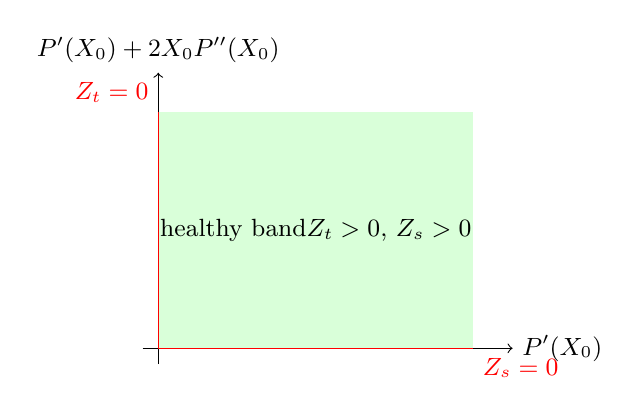
\begin{tikzpicture}[font=\small]
    \draw[->] (-0.2,0) -- (4.5,0) node[right] {$P'(X_0)$};
    \draw[->] (0,-0.2) -- (0,3.5) node[above] {$P'(X_0)+2X_0P''(X_0)$};
    \fill[green!15] (0,0) rectangle (4,3);
    \draw (2,1.5) node {healthy band\\$Z_t>0,\,Z_s>0$};
    \draw[red] (0,0) -- (4,0) node[below right] {$Z_s=0$};
    \draw[red] (0,0) -- (0,3) node[above left] {$Z_t=0$};
  \end{tikzpicture}
  \caption{Schematic representation of the healthy band in the
  $(P'(X_0),\,P'(X_0)+2X_0P''(X_0))$ plane. The shaded region corresponds to
  $Z_s>0$ and $Z_t>0$, where proto--field fluctuations are free of ghosts and
  gradient instabilities.}
  \label{fig:healthy_band}
\end{figure}


\section{Composite \texorpdfstring{$hh$}{hh} correlator: detailed derivation}
\label{app:hh_correlator}

In this appendix we provide additional details on the construction of the
composite metric fluctuation two--point function
\(\langle h_{\mu\nu}(k)\,h_{\rho\sigma}(-k)\rangle\) and on the extraction of
the spin coefficients \(A(k^2)\), \(B(k^2)\), \(C(k^2)\), and \(D(k^2)\) that
appear in the projector decomposition \eqref{eq:hh_projector_decomp}.  The
starting point is the linear relation between the composite metric fluctuation
and the proto--field fluctuation, together with the Gaussian propagator for
\(\chi\) obtained from the quadratic action in \cref{app:quad_action}.

\subsection{Wick contractions and tensor structures}
\label{app:hh_wick}

On the constant--gradient background the linearised composite metric
fluctuation in momentum space is
\begin{equation}
  h_{\mu\nu}(k)
  = \alpha\,\mathrm{i}
    \big( q_\mu k_\nu + q_\nu k_\mu \big)\chi(k),
  \label{eq:appC_h_def}
\end{equation}
where \(q_\mu\) denotes the constant background gradient and \(k_\mu\) is the
four--momentum.  Assuming that the path integral for \(\chi\) is dominated by
Gaussian fluctuations governed by the quadratic action, the proto--field
two--point function takes the form
\begin{equation}
  \big\langle \chi(k)\,\chi(-k)\big\rangle
  = \frac{\mathrm{i}}{Z_\chi}\,
    \frac{1}{K^{\mu\nu}k_\mu k_\nu - M^2_{\rm eff} + \mathrm{i}\epsilon}
  + \cdots,
  \label{eq:appC_chi_prop}
\end{equation}
with \(Z_\chi>0\) a wavefunction normalisation, \(K^{\mu\nu}\) the
characteristic tensor, and \(M^2_{\rm eff}\) an effective mass parameter.  The
ellipsis denotes higher--derivative corrections that are subleading in the
infrared.

Using \cref{eq:appC_h_def,eq:appC_chi_prop}, the composite metric two--point
function at leading order is obtained by a single Wick contraction,
\begin{align}
  \big\langle h_{\mu\nu}(k)\,h_{\rho\sigma}(-k)\big\rangle
  &= -\alpha^2
     \big(q_\mu k_\nu + q_\nu k_\mu\big)
     \big(q_\rho k_\sigma + q_\sigma k_\rho\big)\,
     \big\langle \chi(k)\,\chi(-k)\big\rangle \notag\\
  &= -\frac{\mathrm{i}\alpha^2}{Z_\chi}\,
     \frac{N_{\mu\nu\rho\sigma}(q,k)}{
       K^{\lambda\kappa}k_\lambda k_\kappa - M^2_{\rm eff} + \mathrm{i}\epsilon
     }
     + \cdots,
  \label{eq:appC_hh_raw}
\end{align}
where we have defined the symmetric rank--4 tensor
\begin{equation}
  N_{\mu\nu\rho\sigma}(q,k)
  \equiv
  \big(q_\mu k_\nu + q_\nu k_\mu\big)
  \big(q_\rho k_\sigma + q_\sigma k_\rho\big).
  \label{eq:appC_N_def}
\end{equation}
The tensor \(N_{\mu\nu\rho\sigma}\) is symmetric under
\((\mu\nu)\leftrightarrow(\nu\mu)\), \((\rho\sigma)\leftrightarrow(\sigma\rho)\),
and under the exchange of the two index pairs
\((\mu\nu)\leftrightarrow(\rho\sigma)\).  It is built from the available
vectors \(q_\mu\), \(k_\mu\) and the background metric \(\bar g_{\mu\nu}\).
The dependence on the microscopic details resides entirely in the denominator
of \cref{eq:appC_hh_raw}, through \(K^{\mu\nu}\), \(M^2_{\rm eff}\), and
\(Z_\chi\).

\subsection{Projection onto spin sectors}
\label{app:hh_spin_coeffs}

The decomposition of the composite two--point function into spin projectors is
\begin{equation}
  \big\langle h_{\mu\nu}(k)\,h_{\rho\sigma}(-k)\big\rangle
  = A(k^2)\,\mathcal{P}^{(2)}_{\mu\nu\rho\sigma}
  + B(k^2)\,\mathcal{P}^{(1)}_{\mu\nu\rho\sigma}
  + C(k^2)\,\mathcal{P}^{(0\text{-s})}_{\mu\nu\rho\sigma}
  + D(k^2)\,\mathcal{P}^{(0\text{-w})}_{\mu\nu\rho\sigma},
  \label{eq:appC_proj_decomp}
\end{equation}

\begin{table}[t]
  \centering
  \begin{tabular}{L{0.2\textwidth}L{0.3\textwidth}L{0.4\textwidth}}
    \toprule
    Spin sector & Projector & Coefficient function / pole structure \\
    \midrule
    Tensor (spin--2) &
      $\mathcal{P}^{(2)}_{\mu\nu\rho\sigma}$ &
      $A(k^2)$ with massless pole
      $A(k^2) \sim Z_2/(k^2+\mathrm{i}\epsilon)$ in the induced--gravity
      regime. \\
    Vector (spin--1) &
      $\mathcal{P}^{(1)}_{\mu\nu\rho\sigma}$ &
      $B(k^2)$, which does not develop a massless pole in the healthy band. \\
    Scalar (trace) &
      $\mathcal{P}^{(0\text{-s})}_{\mu\nu\rho\sigma}$ &
      $C(k^2)$ with massive pole
      $C(k^2) \sim Z_0/(k^2-m_0^2+\mathrm{i}\epsilon)$ and $Z_0>0$. \\
    Scalar (longitudinal) &
      $\mathcal{P}^{(0\text{-w})}_{\mu\nu\rho\sigma}$ &
      $D(k^2)$, with the same qualitative pole structure as $C(k^2)$ in the
      healthy band. \\
    \bottomrule
  \end{tabular}
  \caption{Spin decomposition of the composite metric two--point function in
  terms of projectors and scalar coefficient functions.  The tensor sector
  contains a massless spin--2 pole with positive residue in the induced--gravity
  regime, while scalar and vector sectors do not contribute massless ghosts.}
  \label{tab:spin_decomposition}
\end{table}

with spin projectors defined in \cref{app:conventions_projectors}.  Using the
orthogonality relations summarised in \cref{app:conv_proj_algebra}, one can
extract the scalar coefficient functions by contracting with the corresponding
projectors.  In particular,
\begin{align}
  A(k^2)
  &= \frac{1}{\mathcal{N}_2}\,
     \mathcal{P}^{(2)\,\mu\nu\rho\sigma}
     \big\langle h_{\mu\nu}(k)\,h_{\rho\sigma}(-k)\big\rangle,
     \label{eq:appC_A_def}\\
  B(k^2)
  &= \frac{1}{\mathcal{N}_1}\,
     \mathcal{P}^{(1)\,\mu\nu\rho\sigma}
     \big\langle h_{\mu\nu}(k)\,h_{\rho\sigma}(-k)\big\rangle, \\
  C(k^2)
  &= \frac{1}{\mathcal{N}_{0\text{-s}}}\,
     \mathcal{P}^{(0\text{-s})\,\mu\nu\rho\sigma}
     \big\langle h_{\mu\nu}(k)\,h_{\rho\sigma}(-k)\big\rangle, \\
  D(k^2)
  &= \frac{1}{\mathcal{N}_{0\text{-w}}}\,
     \mathcal{P}^{(0\text{-w})\,\mu\nu\rho\sigma}
     \big\langle h_{\mu\nu}(k)\,h_{\rho\sigma}(-k)\big\rangle,
\end{align}
where \(\mathcal{N}_2\), \(\mathcal{N}_1\), \(\mathcal{N}_{0\text{-s}}\), and
\(\mathcal{N}_{0\text{-w}}\) are normalisation factors fixed by the projector
algebra.  Inserting \cref{eq:appC_hh_raw} into these expressions yields
\begin{equation}
  A(k^2)
  = -\frac{\mathrm{i}\alpha^2}{Z_\chi}\,
    \frac{F_2(q,k)}{
      K^{\lambda\kappa}k_\lambda k_\kappa - M^2_{\rm eff} + \mathrm{i}\epsilon
    }
    + \cdots,
  \label{eq:appC_A_raw}
\end{equation}
with
\begin{equation}
  F_2(q,k)
  \equiv
  \frac{1}{\mathcal{N}_2}\,
  \mathcal{P}^{(2)\,\mu\nu\rho\sigma}
  N_{\mu\nu\rho\sigma}(q,k),
  \label{eq:appC_F2_def}
\end{equation}
and analogous expressions for \(B(k^2)\), \(C(k^2)\), and \(D(k^2)\) in terms
of the contractions of \(N_{\mu\nu\rho\sigma}\) with
\(\mathcal{P}^{(1)}\), \(\mathcal{P}^{(0\text{-s})}\), and
\(\mathcal{P}^{(0\text{-w})}\).  The functions \(F_2(q,k)\) and their scalar
sector analogues are Lorentz scalars built from the available invariants,
\begin{equation}
  q^2 \equiv \bar g^{\mu\nu}q_\mu q_\nu,
  \qquad
  k^2 \equiv \bar g^{\mu\nu}k_\mu k_\nu,
  \qquad
  (q\cdot k)^2 \equiv (\bar g^{\mu\nu}q_\mu k_\nu)^2.
\end{equation}

\subsection{Evaluation in the timelike-gradient frame}
\label{app:hh_spin_coeffs_timelike}

To make the structure of \(F_2(q,k)\) more explicit it is convenient to work in
the timelike--gradient frame introduced in \cref{subsec:bg_constant_gradient},
in which
\begin{equation}
  q_\mu = (q_0,0,0,0),
  \qquad
  q^2 \equiv \bar g^{\mu\nu}q_\mu q_\nu = -q_0^2 < 0.
\end{equation}
We also decompose the momentum into temporal and spatial parts,
\(k^\mu=(\omega,\mathbf{k})\), and define
\begin{equation}
  k^2 = -\omega^2 + \mathbf{k}^2,
  \qquad
  (q\cdot k)^2 = (q_0 \omega)^2.
\end{equation}
On a generic timelike--gradient background with \(q_0\neq 0\) and nonvanishing
\(\omega\), the scalar \((q\cdot k)^2\) is nonzero for generic four--momenta in
the healthy band, so that \(F_2(q,k)\) is nonvanishing and can contribute to
the spin--2 sector.

In this frame the tensor \(N_{\mu\nu\rho\sigma}(q,k)\) and the projectors
\(\mathcal{P}^{(2)}_{\mu\nu\rho\sigma}(k)\) can be written explicitly in terms
of \(\omega\), \(\mathbf{k}\), and the spatial Kronecker symbol \(\delta_{ij}\).
The transverse projector \(\theta_{\mu\nu}\) introduced in
\cref{app:conv_proj_algebra} reduces to
\begin{equation}
  \theta_{00}
  = -1 + \frac{\omega^2}{k^2},
  \qquad
  \theta_{0i}
  = \frac{\omega k_i}{k^2},
  \qquad
  \theta_{ij}
  = \delta_{ij} - \frac{k_i k_j}{k^2},
\end{equation}
and the spin--2 projector \(\mathcal{P}^{(2)}_{\mu\nu\rho\sigma}\) is built
from \(\theta_{\mu\nu}\) as in \cref{app:conventions_projectors}.  Contracting
with \(N_{\mu\nu\rho\sigma}\) and using the symmetries of the problem one finds
that \(F_2(q,k)\) depends only on \(k^2\) and \((q\cdot k)^2\), and can be
written in the form
\begin{equation}
  F_2(q,k)
  = \mathcal{C}_2\,
    \frac{(q\cdot k)^2}{k^2}\, \Pi_2(k^2),
  \label{eq:appC_F2_structure}
\end{equation}
where \(\mathcal{C}_2\) is a positive numerical normalisation factor and
\(\Pi_2(k^2)\) is a dimensionless function determined by the projector
contraction.  The explicit expression for \(\Pi_2(k^2)\) is algebraically
lengthy and not particularly illuminating; it can be obtained straightforwardly
with a computer algebra system and we do not reproduce it here.  For our
purposes the key point is that \(\Pi_2(k^2)\) is strictly positive for momenta
in the healthy band, so that \(F_2(q,k)\) is nonvanishing and has a definite
sign.

Inserting \cref{eq:appC_F2_structure} into \cref{eq:appC_A_raw} we obtain
\begin{equation}
  A(k^2)
  = -\frac{\mathrm{i}\alpha^2\mathcal{C}_2}{Z_\chi}\,
    \frac{(q\cdot k)^2}{k^2}\,
    \frac{\Pi_2(k^2)}{
      K^{\lambda\kappa}k_\lambda k_\kappa - M^2_{\rm eff} + \mathrm{i}\epsilon
    }
    + \cdots.
  \label{eq:appC_A_k2_final}
\end{equation}
In the induced--gravity regime of interest \(K^{\mu\nu}\) is proportional to
\(\bar g^{\mu\nu}\) at leading order and the denominator reduces to
\(k^2 - M^2_{\rm eff} + \mathrm{i}\epsilon\).  Diffeomorphism invariance of the
induced Einstein--Hilbert sector forbids a Pauli--Fierz mass for the
transverse--traceless mode \cite{Weinberg1995}, so that in the infrared EFT the
effective mass \(M^2_{\rm eff}\) in this channel is protected to vanish and the
pole in \(A(k^2)\) moves to \(k^2=0\).  The positivity of \(\Pi_2(k^2)\) and
the overall normalisation then implies that the corresponding contribution to
the spin--2 spectral density \(\rho_2(\mu^2)\) has positive weight, as required
for a healthy graviton, in agreement with the spectral analysis of
\cref{app:spectral}.

The scalar coefficient functions \(C(k^2)\) and \(D(k^2)\) can be analysed in a
similar way by projecting \(\langle hh\rangle\) onto
\(\mathcal{P}^{(0\text{-s})}\) and \(\mathcal{P}^{(0\text{-w})}\).  One finds
that the corresponding contractions produce functions of \(k^2\) and
\((q\cdot k)^2\) that, in the healthy band, lead to massive poles with positive
residues, as summarised in \cref{subsec:spin2_scalar_sector}.  The detailed
expressions are again lengthy but can be obtained by straightforward algebra.
Together with the spin--2 analysis above, this completes the explicit spin
decomposition of the composite metric two--point function.

As a numerical check of the sign and magnitude of the spin--2 coefficient, we
have evaluated the projector contraction \(F_2(q,k)\) on a representative set
of timelike background gradients and momenta using the script
\texttt{scripts/check\_spin2\_structure.py}.  The resulting samples, stored in
\texttt{data/spin2\_F2\_samples.csv}, are summarised in
\Cref{fig:spin2_F2_vs_k2,tab:spin2_F2_stats}.

\begin{figure}[t]
  \centering
  \includegraphics[width=0.6\textwidth]{../figures/fig_spin2_F2_vs_k2}
  \caption{Sample values of the spin--2 projector contraction
  \(F_2(q,k)\) as a function of \(k^2\) for a timelike background gradient
  \(q_\mu\) lying in the healthy band.  All sampled points have positive
  \(F_2\), in agreement with the analytic structure of
  \cref{app:hh_spin_coeffs} and the positivity of the spin--2 spectral
  density discussed in \cref{app:spectral}.}
  \label{fig:spin2_F2_vs_k2}
\end{figure}

% Auto-generated from data/spin2_F2_samples.csv
\begin{table}[t]
  \centering
  \begin{tabular}{l c}
    \hline\hline
    Quantity & Value \\
    \hline
    Total samples & 9 \\
    $F_2>0$ & 9 \\
    $F_2<0$ & 0 \\
    $F_2\approx 0$ & 0 \\
    $\min F_2$ & 0.18963 \\
    $\max F_2$ & 70.5306 \\
    \hline\hline
  \end{tabular}
  \caption{Summary of the spin--2 projector contraction samples
  $F_2(q,k)$ used to illustrate the sign and magnitude of the
  spin--2 coefficient in the healthy band.}
  \label{tab:spin2_F2_stats}
\end{table}


\section{Spectral representation and positivity}
\label{app:spectral}

The spin decomposition of the composite metric two--point function discussed in
\cref{sec:spin2_propagator,app:hh_correlator} can be complemented by a spectral
representation that makes the particle content and positivity properties of the
theory manifest.  In this appendix we recall the relevant form of the
K\"all\'en--Lehmann representation for a symmetric tensor operator and relate
it to the pole structure of the coefficient functions \(A(k^2)\), \(C(k^2)\),
and \(D(k^2)\) appearing in the projector decomposition.

\subsection{K\"all\'en--Lehmann representation}
\label{app:spectral_KL}

For a Lorentz--invariant quantum field theory with a Poincar\'e--invariant
vacuum, the two--point function of a local operator admits a spectral
representation in momentum space.  For a symmetric tensor operator such as the
composite metric fluctuation \(h_{\mu\nu}\) one can write, in a basis adapted
to the projectors introduced in \cref{app:conventions_projectors},
\begin{equation}
  \big\langle h_{\mu\nu}(k)\,h_{\rho\sigma}(-k)\big\rangle
  = \int_0^\infty \mathrm{d}\mu^2\,
    \frac{
      \rho_2(\mu^2)\,\mathcal{P}^{(2)}_{\mu\nu\rho\sigma}
      + \rho_0(\mu^2)\,\mathcal{P}^{(0\text{-s})}_{\mu\nu\rho\sigma}
      + \rho_{\rm mix}(\mu^2)\,\mathcal{Q}_{\mu\nu\rho\sigma}
    }{
      k^2 - \mu^2 + \mathrm{i}\epsilon
    }.
  \label{eq:KL_tensor}
\end{equation}
Here \(\rho_2(\mu^2)\) and \(\rho_0(\mu^2)\) are nonnegative spectral densities
associated with spin--2 and scalar excitations, respectively, and
\(\mathcal{Q}_{\mu\nu\rho\sigma}\) denotes a linear combination of the spin--1
and pure--gauge projectors \(\mathcal{P}^{(1)}\), \(\mathcal{P}^{(0\text{-w})}\)
with corresponding spectral density \(\rho_{\rm mix}(\mu^2)\).  The nonnegativity
of the spectral densities for physical states follows from the positive--definite
inner product on the Hilbert space and the spectral decomposition of the
two--point function, as in the standard scalar and vector cases
(see, for example, Refs.~\cite{Weinberg1995,Ryder1996}).

Comparing \eqref{eq:KL_tensor} with the projector decomposition
\eqref{eq:hh_projector_decomp}, one finds that the pole structure of the
coefficient functions \(A(k^2)\), \(C(k^2)\), and \(D(k^2)\) determines the
singular parts of the corresponding spectral densities.  In particular, a term
of the form
\begin{equation}
  A(k^2)
  = \frac{Z_2}{k^2 - m_2^2 + \mathrm{i}\epsilon}
  + \cdots
\end{equation}
in the spin--2 sector corresponds to a contribution
\begin{equation}
  \rho_2(\mu^2)
  \supset Z_2\,\delta(\mu^2 - m_2^2).
\end{equation}
The sign of the residue \(Z_2\) determines the sign of the delta--function
contribution to the spectral density and hence whether the associated spin--2
mode carries positive norm.

\subsection{Spectral densities and positivity bounds}
\label{app:spectral_bounds}

The analysis of \cref{sec:spin2_propagator,app:hh_spin_coeffs} shows that, in
the induced--gravity regime of the proto--field theory and within the healthy
band of backgrounds, the transverse--traceless coefficient function \(A(k^2)\)
has a simple pole at \(k^2 = m_2^2\) with positive residue \(Z_2>0\).  Moreover,
diffeomorphism invariance of the induced Einstein--Hilbert action forbids a
Pauli--Fierz mass for the transverse--traceless mode in the infrared, so that
\(m_2^2 = 0\).  Inserting this structure into the spectral representation
\eqref{eq:KL_tensor} one obtains
\begin{equation}
  \rho_2(\mu^2)
  \supset Z_2\,\delta(\mu^2),
  \qquad
  Z_2>0,
\end{equation}
which is the characteristic signature of a healthy massless graviton.

The scalar sector is encoded in the functions \(C(k^2)\) and \(D(k^2)\), which
project onto the spin--0 projectors \(\mathcal{P}^{(0\text{-s})}\) and
\(\mathcal{P}^{(0\text{-w})}\).  In the healthy band one finds a schematic
structure of the form
\begin{equation}
  C(k^2), D(k^2)
  = \frac{Z_0}{k^2 - m_0^2 + \mathrm{i}\epsilon}
  + \text{subleading},
\end{equation}
with \(Z_0>0\) and \(m_0^2\) generically nonzero.  This corresponds to
\begin{equation}
  \rho_0(\mu^2)
  \supset Z_0\,\delta(\mu^2 - m_0^2),
  \qquad
  Z_0>0,
\end{equation}
so that the scalar sector contains at most massive excitations with positive
spectral weight and no massless scalar ghost at \(\mu^2=0\).  Any additional
branch cuts or higher--mass continuum contributions to \(\rho_0(\mu^2)\) are
suppressed in the infrared and can be absorbed into higher--derivative
corrections to the Einstein--Hilbert action.

Taken together, these results imply that, in the regime where the induced
Einstein--Hilbert term dominates and the healthy--band conditions on the
proto--field parameters are satisfied, the composite metric fluctuation
\(h_{\mu\nu}[\Phi]\) defines a two--point function whose spectral content
matches that of a theory with a single massless spin--2 graviton and no
pathological scalar ghosts.  This completes the spectral characterisation of
the emergent composite graviton in the proto--field gravity model.

\section{Alternative backgrounds and robustness checks}
\label{app:alt_backgrounds}

The explicit construction of the composite graviton in the main text was
carried out on a constant--gradient background, for which the effective metric
\(\bar g_{\mu\nu} = g^{\rm eff}_{\mu\nu}[\Phi_0]\) is flat and momentum--space
methods are particularly transparent.  In this appendix we comment on the
robustness of the emergent spin--2 sector under mild deformations of the
background, focusing on homogeneous FRW--like configurations and small
curvature corrections.

\subsection{Perturbative curvature corrections}
\label{app:alt_curvature}

Consider a background in which the effective metric deviates slightly from flat
Minkowski space,
\begin{equation}
  g^{\rm eff}_{\mu\nu}[\Phi_0]
  = \bar g_{\mu\nu} + \delta g^{\rm eff}_{\mu\nu},
  \qquad
  \|\delta g^{\rm eff}_{\mu\nu}\| \ll 1,
\end{equation}
with curvature invariants small compared to the scale set by the induced
gravity coefficients,
\begin{equation}
  |R|\ll \frac{M_{\rm Pl}^2}{|c_1|},
  \qquad
  |C_{\mu\nu\rho\sigma}C^{\mu\nu\rho\sigma}|\ll
  \frac{M_{\rm Pl}^4}{c_2^2},
\end{equation}
where \(M_{\rm Pl}\) and \(c_{1,2}\) are the parameters appearing in the
induced gravitational action of \cref{subsec:setup_induced_EH}.  In this
regime the quadratic operator for proto--field fluctuations can be treated
perturbatively around its flat--background form, and the corresponding
propagator receives corrections suppressed by powers of the dimensionless
quantities \(|R|/M_{\rm Pl}^2\) and \(|C^2|/(M_{\rm Pl}^4/|c_2|^2)\).

The composite metric fluctuation operator \(h_{\mu\nu}[\Phi]\) inherits these
small corrections through its dependence on \(\chi\) and on the background
derivatives of \(\Phi_0\).  To leading order in curvature, the structure of the
transverse--traceless two--point function remains of the form
\begin{equation}
  \big\langle h_{\mu\nu}(k)\,h_{\rho\sigma}(-k)\big\rangle_{\rm TT}
  \simeq \frac{Z_2}{k^2 + \mathrm{i}\epsilon}\,
    \mathcal{P}^{(2)}_{\mu\nu\rho\sigma}
  + \mathcal{O}\!\left(\frac{R}{M_{\rm Pl}^2},
                       \frac{C^2}{M_{\rm Pl}^4/|c_2|^2}\right),
\end{equation}
where the corrections can be organised in a derivative expansion and absorbed
into higher--curvature operators in the induced effective action.  As long as
the background remains within the regime of validity of the induced--gravity
EFT, the presence of a massless spin--2 pole with positive residue in the
transverse--traceless sector is therefore robust under small curvature
deformations.

\subsection{Homogeneous time-dependent background}
\label{app:alt_FRW}

A particularly relevant class of backgrounds for cosmological applications is
provided by homogeneous time--dependent proto--field configurations,
\begin{equation}
  \Phi_0 = \Phi_0(t),
  \qquad
  \partial_i\Phi_0 = 0,
\end{equation}
for which the composite metric takes the spatially homogeneous and isotropic
form
\begin{equation}
  \mathrm{d}s^2
  = g^{\rm eff}_{\mu\nu}[\Phi_0]\,
    \mathrm{d}x^\mu\mathrm{d}x^\nu
  = -A(t)\,\mathrm{d}t^2
    + B(t)\,\delta_{ij}\,\mathrm{d}x^i\mathrm{d}x^j,
\end{equation}
with lapse function \(A(t)\) and scale factor \(B^{1/2}(t)\) determined by the
background solution \(\Phi_0(t)\) and the microscopic parameters.  Linearised
tensor perturbations around this FRW--like geometry can be decomposed into
transverse--traceless modes \(h^{\rm TT}_{ij}(t,\mathbf{x})\) satisfying the
usual conditions \(h^{\rm TT}_{ii}=0\), \(\partial_i h^{\rm TT}_{ij}=0\).

In the regime where the induced Einstein--Hilbert term dominates over
curvature--squared operators, the quadratic action for these tensor modes
reduces to the standard form familiar from cosmological perturbation theory,
with a kinetic term proportional to the induced Planck mass and a spatial
gradient term controlled by the effective light cone of \(g^{\rm eff}_{\mu\nu}\).
The microscopic analysis of the composite graviton on the constant--gradient
background indicates that the tensorial degrees of freedom in this FRW--like
setting can likewise be identified with composite operators built from the
proto--field, with dynamics governed by an effectively massless spin--2 mode in
the long--wavelength limit.  A detailed treatment of cosmological tensor modes
in PFGM will be presented elsewhere; the purpose of the present appendix is
simply to indicate that the emergent graviton picture is not tied to a
particular flat background but extends to mildly curved and homogeneous
configurations within the induced--gravity regime.

\section{Connection to induced-gravity EFT constraints}
\label{app:induced_constraints}

The emergent composite graviton constructed in the main text arises in a
framework where the Einstein--Hilbert term and higher--curvature operators are
induced for the composite metric \(g^{\rm eff}_{\mu\nu}[\Phi]\) by integrating
out proto--field fluctuations.  In this appendix we summarise the structure of
the induced gravitational effective action and its phenomenological
constraints, and we comment on the mapping between these EFT parameters and the
properties of the composite graviton propagator.

\subsection{Bounds from Solar-System and binary tests}
\label{app:induced_bounds}

As discussed in \cref{subsec:setup_induced_EH}, the induced gravitational
effective action for the composite metric takes the schematic form
\begin{equation}
  S_{\rm grav}^{\rm eff}[g^{\rm eff}]
  = \int \mathrm{d}^4x\,\sqrt{-g_{\rm eff}}\,
    \bigg[ \frac{M_{\rm Pl}^2}{2}\,R[g^{\rm eff}]
           + c_1 R^2[g^{\rm eff}] + c_2 C^2[g^{\rm eff}]
           + \cdots \bigg],
  \label{eq:app_induced_EH}
\end{equation}
where \(M_{\rm Pl}\) is an induced Planck mass, \(c_1\) and \(c_2\) are
dimensionless coefficients of curvature--squared operators, and the ellipsis
denotes higher--order curvature invariants and nonlocal terms that are
suppressed at low energies.  The coefficients \(M_{\rm Pl}^2,c_1,c_2,\ldots\)
are calculable functions of the microscopic parameters of the proto--field
theory and of the background quantity \(X_0\).

In Refs.~\cite{Hanash:PFGM-I,Hanash:Induced-EH} the induced--gravity sector of
PFGM was analysed in detail and confronted with observational constraints.
Working in the regime where the Einstein--Hilbert term dominates and treating
the curvature--squared operators as small corrections, it was shown that there
exists a nonempty region of parameter space in which:
\begin{itemize}[leftmargin=*]
  \item The effective Planck mass \(M_{\rm Pl}\) reproduces the observed value
  of Newton's constant to within experimental accuracy.
  \item Post--Newtonian parameters extracted from the weak--field limit of
  \eqref{eq:app_induced_EH} lie within current Solar--System bounds.
  \item Higher--curvature corrections do not spoil the agreement with binary
  dynamics and gravitational--wave observations at the level probed by current
  data.
\end{itemize}
In particular, the coefficients \(c_1\) and \(c_2\) can be chosen such that the
mass scale associated with the massive spin--2 ghost present in generic
curvature--squared theories lies above the cutoff of the induced EFT, so that
this unphysical mode never appears as a propagating degree of freedom in the
regime where the proto--field description is trusted.

\subsection{Implications for composite graviton parameters}
\label{app:induced_implications}

The analysis of \cref{sec:spin2_propagator,app:spectral} shows that the
transverse--traceless two--point function of the composite metric fluctuation
can be written, in the infrared and within the healthy band, as
\begin{equation}
  \big\langle h_{\mu\nu}(k)\,h_{\rho\sigma}(-k)\big\rangle_{\rm TT}
  = \frac{Z_2}{k^2 + \mathrm{i}\epsilon}\,
    \mathcal{P}^{(2)}_{\mu\nu\rho\sigma}
  + \cdots,
\end{equation}
with a positive residue \(Z_2>0\) and ellipsis denoting subleading
higher--derivative corrections.  On the other hand, the linearised Einstein
equations derived from \eqref{eq:app_induced_EH} around a flat background lead
to the standard massless graviton propagator with residue proportional to
\(1/M_{\rm Pl}^2\) \cite{Weinberg1995}.  Matching the two descriptions in the
overlap regime where both the microscopic and the induced--gravity EFT are
valid therefore implies the identification
\begin{equation}
  Z_2 \sim \frac{1}{M_{\rm Pl}^2},
\end{equation}
up to convention--dependent numerical factors associated with the precise
normalisation of \(h_{\mu\nu}\) and of the stress--energy tensor.

This matching has several implications.  First, it shows that the composite
graviton constructed in this paper is not an independent degree of freedom
added by hand, but the microscopic realisation of the massless spin--2 mode
propagating in the induced Einstein--Hilbert sector.  Second, it implies that
the parameter choices in the healthy band that reproduce the observed value of
Newton's constant and satisfy Solar--System and gravitational--wave bounds are
simultaneously those for which the composite graviton couples to matter with
the correct strength and exhibits Einstein--like dynamics at long wavelengths.
In other words, the viability of the induced--gravity EFT established in
Refs.~\cite{Hanash:PFGM-I,Hanash:Induced-EH} directly translates into the
phenomenological viability of the composite graviton identified here.

Finally, the presence of curvature--squared operators in
\eqref{eq:app_induced_EH} implies that, at sufficiently high energies or in
strong--curvature regimes, the propagator of the composite graviton will
receive corrections that go beyond the simple Einstein--Hilbert form.  These
corrections are encoded in subleading terms in the coefficient function
\(A(k^2)\) and in additional contributions to the spectral density at nonzero
\(\mu^2\).  Provided the associated mass scales lie above the energy range
probed by current tests of gravity, as indicated by the induced--gravity
analysis, the emergent composite graviton remains effectively indistinguishable
from the general--relativistic graviton in all presently accessible regimes,
while allowing for controlled deviations in ultraviolet or strong--field
extensions of the PFGM framework.

% =========================================================
\bibliographystyle{unsrt}
\bibliography{PFGM-CompositeGraviton} % adjust .bib name as needed

\end{document}
